% Pre-ambulo
\documentclass[a4paper, 12pt]{abnt}

\usepackage[brazil]{babel}
\usepackage[latin1]{inputenc}
\usepackage[T1]{fontenc}
\usepackage{dsfont}
\usepackage{amssymb,amsmath}
\usepackage{multirow}
\usepackage[alf]{abntcite}
\usepackage[pdftex]{color, graphicx}
\usepackage{colortbl}
\usepackage{url}
\usepackage{abnt-alf}
\usepackage{abntcite}
\usepackage{algorithm}
\usepackage{algorithmic}
\usepackage{makecell}

%\usepackage{alg}
%\usepackage{hyperref}
% Redefinicao de instrucoes
\floatname{algorithm}{Algoritmo}
\renewcommand{\algorithmicrequire}{\textbf{Entrada:}}
\renewcommand{\algorithmicensure}{\textbf{Sa�da:}}
\renewcommand{\algorithmicend}{\textbf{fim}}
\renewcommand{\algorithmicif}{\textbf{se}}
\renewcommand{\algorithmicthen}{\textbf{ent�o}}
\renewcommand{\algorithmicelse}{\textbf{sen�o}}
\renewcommand{\algorithmicfor}{\textbf{para}}
\renewcommand{\algorithmicforall}{\textbf{para todo}}
\renewcommand{\algorithmicdo}{\textbf{fa�a}}
\renewcommand{\algorithmicwhile}{\textbf{enquanto}}
\renewcommand{\algorithmicloop}{\textbf{loop}}
\renewcommand{\algorithmicrepeat}{\textbf{repetir}}
\renewcommand{\algorithmicuntil}{\textbf{at� que}}
\renewcommand{\algorithmiccomment}[1]{\% #1}


% Definicao da lista de simbolos
% \simb[entrada na lista de simbolos]{simbolo}:
% Escreve o simbolo no texto e uma entrada na lista de simbolos.
% Se o parametro opcional e omitido, usa-se o parametro obrigatorio.
\newcommand{\simb}[2][]
{%
	\ifthenelse{\equal{#1}{}}
	{\addcontentsline{los}{simbolo}{#2}}
	{\addcontentsline{los}{simbolo}{#1}}#2
}
% Para aceitar comandos com @ (at) no nome
\makeatletter 
% \listadesimbolos: comando que imprime a lista de simbolos
\newcommand{\listadesimbolos}
{
	\pretextualchapter{Lista de s�mbolos}
	{\setlength{\parindent}{0cm}
	\@starttoc{los}}
}
% Como a entrada sera impressa
\newcommand\l@simbolo[2]{\par #1}
\makeatother


% Definicao da lista de abreviaturas e siglas
% \abrv[entrada na lista de simbolos]{abreviatura}:
% Escreve a sigla/abreviatura no texto e uma entrada na lista de abreviaturas e siglas.
% Se o parametro opcional e omitido, usa-se o parametro obrigatorio.
\newcommand{\abrv}[2][]
{%
	\ifthenelse{\equal{#1}{}}
	{\addcontentsline{loab}{abreviatura}{#2}}
	{\addcontentsline{loab}{abreviatura}{#1}}#2
}
% Para aceitar comandos com @ (at) no nome
\makeatletter 
% \listadeabreviaturas: comando que imprime a lista de abreviaturas e siglas
\newcommand{\listadeabreviaturas}
{
	\pretextualchapter{Lista de abreviaturas e siglas}
	{\setlength{\parindent}{0cm}
	\@starttoc{loab}}
}
% Como a entrada sera impressa
\newcommand\l@abreviatura[2]{\par #1}
\makeatother


% \listofalgorithms: comando que imprime a lista de algoritmos
\renewcommand{\listalgorithmname}{Lista de algoritmos}


% Hifeniza��o de palavras feita de forma incorreta pelo LaTeX
\hyphenation{PYTHON ou-tros}


% Inicio do documento
\begin{document}

	\frenchspacing
	
	% Capa (arquivo Includes/Capa.tex)
	
\newcommand*{\captionsource}[2]{%
  \caption[{#1}]{%
    #1%
    \\\hspace{\linewidth}%
    \textbf{Fonte:} #2%
  }%
}
% Capa
% Prote��o externa do trabalho e sobre a qual se imprimem as informa��es indispens�veis 
% � sua identifica��o.

% Especifica��o da capa
\begin{titlepage}
	\begin{center}
		
		% Cabe�alho (n�o deve ser modificado)
		% Cont�m o bras�o da Universidade, o logotipo do Departamento, al�m dos dados
		% relacionados � vincula��o do aluno (Universidade, Centro, Departamento e Curso)
		\begin{minipage}{2cm}
			\begin{center}
				
\includegraphics[width=1.7cm, height=2.0cm]{Imagens/Brasao-UFRN.jpg}
			\end{center}
		\end{minipage}
		\begin{minipage}{11cm}
			\begin{center}
				\begin{espacosimples}
					{\small \textsc{Universidade Federal do Rio Grande do Nort}			\\
							  \textsc{Centro de Ci�ncias Exatas e da Terra}						\\
							  \textsc{Departamento de Inform�tica e Matem�tica Aplicada}	\\
							  \textsc{Bacharelado em Ci�ncia da Computa��o}}
				\end{espacosimples}
			\end{center}
		\end{minipage}
		\begin{minipage}{2cm}
			\begin{center}
				
\includegraphics[width=1.8cm, height=1.5cm]{Imagens/Logotipo-DIMAp.jpg}
			\end{center}
		\end{minipage}
			
		\vspace{6cm}
						
		% T�tulo do trabalho
		{\setlength{\baselineskip}%
		{1.3\baselineskip}
		{\LARGE \textbf{Roomie: uma aplica��o para pr�dios inteligentes baseada na infraestrutura de Internet das Coisas }}\par}
			
		\vspace{4cm}
			
		% Nome do aluno (autor)
		{\large \textbf{Viviane Costa Pinheiro}}
						
		\vspace{7cm}
		
		% Local da institui��o onde o trabalho deve ser apresentado e ano de entrega do mesmo
		Natal-RN\\Maio 2017
	\end{center}
\end{titlepage}

	% Folha de rosto (arquivo Includes/FolhaRosto.tex)
	% Folha de rosto
% Cont�m os elementos essenciais � identifica��o do trabalho.

% T�tulo, nome do aluno e respectivo orientador e filia��o
\titulo{\Large{Roomie: uma aplica��o para pr�dios inteligentes baseada na infraestrutura de Internet das Coisas}}
\autor{Viviane Costa Pinheiro }
\orientador[Orientador(a)]{\par Prof. Me.
Itamir de Morais Barroca Filho
}
\instituicao
{
	Universidade Federal do Rio Grande do Norte -- UFRN \par 
	Departamento de Inform�tica e Matem�tica Aplicada -- DIMAp
}
	
% Natureza do trabalho (n�o deve ser modificada)
\comentario
{
	Monografia de Gradua��o apresentada ao Departamento de Inform�tica e Matem�tica Aplicada do 
	Centro de Ci�ncias Exatas e da Terra da Universidade Federal do Rio Grande do Norte como
	requisito parcial para a obten��o do grau de bacharel em Ci�ncia da Computa��o.
}
		
% Local e data
\local{Natal-RN}
\data{Maio 2017}
	
\folhaderosto	
	
	% Folha de aprovacao (arquivo Includes/FolhaAprovacao.tex)
	% Folha de aprova��o
\begin{folhadeaprovacao}
	\setlength{\ABNTsignthickness}{0.4pt}
	\setlength{\ABNTsignwidth}{10cm}
	
	% Informa��es gerais acerca do trabalho 
	% (nome do autor, t�tulo, institui��o � qual � submetido e natureza)
	\noindent 
	Monografia de Gradua��o sob o t�tulo \textit{Roomie: uma aplica��o para pr�dios inteligentes baseada na infraestrutura de Internet das Coisas} apresentada por 
	Nome do aluno e aceita pelo Departamento de Inform�tica e Matem�tica Aplicada do
	Centro de Ci�ncias Exatas e da Terra da Universidade Federal do Rio Grande do Norte,
	sendo aprovada por todos os membros da banca examinadora abaixo especificada:
		
	% Membros da banca examinadora e respectivas filia��es
	\assinatura
	{
		Titula��o e nome do(a) orientador(a)\\
		{\small Orientador(a)} 															\\ 
		{\footnotesize
			Departamento 																	\\
		  	Universidade
		}
	}
	
	\assinatura
	{
		Titula��o e nome do membro da banca examinadora							\\
		{\small Co-orientador(a), se houver}										\\ 
		{\footnotesize
			Departamento 																	\\
		  	Universidade
		}
	}
		
	\assinatura
	{
		Titula��o e nome do membro da banca examinadora 						 \\ 
		{\footnotesize
			Departamento 																	 \\
		  	Universidade
		}
	}
		
	\assinatura
	{
		Titula��o e nome do membro da banca examinadora 						 \\ 
		{\footnotesize
			Departamento 																	 \\
		  	Universidade
		}
	}
		
	\vfill
	
	\begin{center}
		Natal-RN, data de aprova��o (por extenso).
	\end{center}
\end{folhadeaprovacao}	
	
	% Dedicatoria (arquivo Includes/Dedicatoria.tex)
	% Dedicat�ria

\chapter*{}
\vspace{15cm}
\begin{flushright}
	Homenagem que o autor presta a uma ou mais pessoas.
\end{flushright}
	
	% Agradecimentos (arquivo Includes/Agradecimentos.tex)
	%include{Includes/Agradecimentos}
   
   % Epigrafe (arquivo Includes/Epigrafe.tex)
	%% Ep�grafe (cita��o seguida de indica��o de autoria)

\chapter*{}
\vspace{15cm}
\begin{flushright}
	\textit
	{
		Cita��o
	}\medskip\\ 
	Autor
\end{flushright}
	
	% Resumo em l�ngua vernacula (arquivo Includes/Resumo.tex)
	% Resumo em l�ngua vern�cula
\begin{center}
	{\Large{\textbf{Roomie: uma aplica��o para pr�dios inteligentes baseada na infraestrutura de Internet das Coisas}}}
\end{center}

\vspace{1cm}

\begin{flushright}
	Autor: Viviane Costa Pinheiro\\
	Orientador(a): Prof. Me. Itamir de Barrocas Filho 
\end{flushright}

\vspace{1cm}

\begin{center}
	\Large{\textsc{\textbf{Resumo}}}
\end{center}

\noindent  
Com os avan�os tecnol�gicos dos �ltimos anos e a populariza��o da Internet das Coisas(IoT), hoje em dia � poss�vel desenvolver novas aplica��es que resolvem velhos problemas do nosso cotidiano que antigamente n�o possu�am uma solu��o vi�vel. Uma das �reas que est� sendo bastante explorada nesse novo contexto s�o as aplica��es espec�ficas para pr�dios inteligentes. Dentro dos problemas de gerenciamento de pr�dios, um dos problemas mais recorrentes � o mau uso dos espa�os, em especial das salas de reuni�o. No entanto os softwares tradicionais utilizados para reservas de salas n�o conseguem resolver todas as dificuldades relacionados a ger�ncia desses espa�os, principalmente por n�o se adaptarem ao ambiente no qual est�o inseridos e ao comportamento dos usu�rios em tempo real. Este trabalho tem como principal objetivo  descrever o desenvolvimento de uma aplica��o voltada para reserva de salas de reuni�o, a aplica��o utiliza infraestrutura de IoT para a incorpora��o de dados de sensores na aplica��o de reserva para permitir a adapta��o do sistema ao comportamento dos usu�rios e estados das salas. 
\noindent\textit{Palavras-chave}: Internet das Coisas,Pr�dios Inteligentes, Sistemas de Reserva de Sala.
	
	% Abstract, resumo em l�ngua estrangeira (arquivo Include/Abstract.tex)
	%% Resumo em l�ngua estrangeira (em ingl�s Abstract, em espanhol Resumen, em franc�s R�sum�)
\begin{center}
	{\Large{\textbf{T�tulo do trabalho (em l�ngua estrangeira)}}}
\end{center}

\vspace{1cm}

\begin{flushright}
	Author: Nome do aluno\\
	Advisor: Titula��o e nome do(a) orientador(a)
\end{flushright}

\vspace{1cm}

\begin{center}
	\Large{\textsc{\textbf{Abstract}}}
\end{center}

\noindent O resumo em l�ngua estrangeira (em ingl�s \textit{Abstract}, em espanhol \textit{Resumen}, em franc�s \textit{R�sum�}) � uma vers�o do resumo escrito na l�ngua vern�cula para idioma de divulga��o internacional. Ele deve apresentar as mesmas caracter�sticas do anterior (incluindo as mesmas palavras, isto �, seu conte�do n�o deve diferir do resumo anterior), bem como ser seguido das palavras representativas do conte�do do trabalho, isto �, palavras-chave e/ou descritores, na l�ngua estrangeira. Embora a especifica��o abaixo considere o ingl�s como l�ngua estrangeira (o mais comum), n�o fica impedido a ado��o de outras linguas (a exemplo de espanhol ou franc�s) para reda��o do resumo em l�ngua estrangeira.

\noindent\textit{Keywords}: Keyword 1, Keyword 2, Keyword 3.
	
	% Lista de figuras
	\listoffigures

	% Lista de tabelas
	%\listoftables
	
	% Lista de abreviaturas e siglas
	\listadeabreviaturas
	
	% Lista de algoritmos (se houver)
	% Devem ser inclu�dos os pacotes algorithm e algorithmic
	% \listofalgorithms
	
	% Sum�rio
	\sumario

	% Parte central do trabalho, englobando os cap�tulos que constituem o mesmo
	% Os referidos cap�tulos devem ser organizados dentro do diret�rio "Cap�tulos"

	% Capitulo 1: Introdu��o (arquivo Includes/Introducao.tex)
	% Introdu��o
\chapter{Introdu��o}
No panorama atual da Computa��o, um novo paradigma que surge com cada vez mais for�a nos �ltimos anos,  � a Internet das Coisas ou em ingl�s,  Internet of Things(\abrv[IoT -- Internet of Things]{IoT}). A IoT pode ser definida como uma rede mundial de objetos interconectados e unicamente endere�ados, baseado em protocolos tradicionais de comunica��o \cite{atzori}. Esse novo paradigma traz um novo tipo de relacionamento que antes era baseado apenas em homem-m�quina  e passa tamb�m a ser m�quina-m�quina \cite{tan&wang}. A IoT traz uma possibilidade de dezenas de novas aplica��es para o futuro, focando nas mais diversas �reas, como: transportes, log�stica, ambientes inteligentes, sa�de e aplica��o pessoais entre outras.

Uma das aplica��es que nos �ltimos anos tem ganhado cada vez mais for�a gra�as ao IoT, s�o as aplica��es para smart buildings ou pr�dios inteligentes. Uma das defini��es fornecidas para Smart Building pelo  \cite{harris} , � que um smart building � um pr�dio que possui caracter�sticas mut�veis e possui  a habilidade de se adaptar a mudan�as em ambientes externos e internos a fim de endere�ar problemas de conforto, financeiro e  de consumo de energia. Grande parte das aplica��es de smart building se concentram em proporcionar um gerenciamento mais inteligente dos espa�os f�sicos dos pr�dios, proporcionando redu��o do consumo de energia e tamb�m uma melhor adapta��o do pr�dio a condi��es externas como ilumina��o e temperatura.


\section{Defini��o do Trabalho}
Um dos grandes problemas em grandes pr�dios comerciais hoje em dia � a m� utiliza��o dos espa�os, em especial das salas de reuni�o. E apesar de j� existirem diversos sistemas que abordam o tema do controle de espa�os, poucos possuem a habilidade de serem sens�veis ao ambiente em que est�o inseridos, ou seja, poucos capturam dados e informa��es do ambiente que est�o inseridos para uma tomada futura de decis�o. A falta dessa caracter�stica implica na n�o detec��o de alguns problemas comuns na utiliza��o desses espa�os. Os problemas comumente n�o detectados s�o:

\begin{itemize}
	\item \textit{No-show}. Acontece quando a sala � reservada, no entanto a reuni�o acaba sendo cancelada mas a reserva n�o. Esse comportamento n�o � t�o incomum  quanto parece, pois aproximadamente 40\% das reservas acabam em no-show \cite{duncan}.  

	\item Reservas maiores que reuni�es. Um comportamento comum dos usu�rios que utilizam sistemas de reservas de salas � reservar um tempo maior que o necess�rio, para que n�o corram riscos de ficar sem sala. No entanto normalmente a reuni�o dura menos tempo que o reservado mas sala continua com o status de ocupada no sistema, pois n�o � poss�vel a identifica��o do fim da reuni�o \cite{tran}. 
	\item O ''roubo'' de salas. Essa situa��o ocorre quando alguns usu�rios desconsideram as reservas previamente feitas para a sala e utilizam o espa�o sem ter realizado alguma reserva. Como normalmente n�o existe um mecanismo de autentica��o para identificar o usu�rio que realizou a tarefa essa � uma situa��o que acaba sendo bastante comum.


\end{itemize}
Esses problemas de mau uso e inadequa��o dos sistemas a realidade dos pr�dios, acaba saindo caro para as empresas, pois ser�o necess�rias um n�mero muito superior de salas de reuni�o para suprir essa lacuna de salas sendo usadas ineficientemente.

\section{Objetivos}

Este trabalho tem o objetivo geral descrever o desenvolvimento de uma aplica��o de Smart Building utilizando a infraestrutura da Internet das Coisas, aplica��o � denominada Roomie. Os objetivos espec�ficos  que querem ser alcan�ados ao final do texto s�o:
\begin{itemize}
	\item Relatar o desenvolvimento de uma aplica��o baseada na arquitetura de IoT, desde sua documenta��o at� sua implementa��o;
	\item Realizar uma compara��o das tecnologias atuais que possam ser usadas para desenvolver esse tipo de aplica��o.
	\item Identificar as poss�veis dificuldades e limita��es fornecidas pelas ferramentas atuais.
\end{itemize}	

\section{Organiza��o do Trabalho}

O trabalho � organizado em se��es, que est�o organizadas da seguinte maneira:
\begin{itemize}
	\item Na se��o 2 s�o apresentadas as tecnologias que foram utilizadas no desenvolvimento da aplica��o, 
	\item Na se��o 3 temos compara��o com outras aplica��es que tem finalidade similares e abordam o tema de controle de espa�os em pr�dios.
	\item Na se��o 4 � descrita o desenvolvimento da ferramenta, requisitos, arquitetura. implementa��o de testes da aplica��o.
	\item A se��o 5, retrata as considera��es finais do trabalho e abre espa�o para discuss�o sobre poss�veis trabalhos futuros baseados no presente trabalho de conclus�o.
\end{itemize}	

	
	% Capitulo 2: Segundo cap�tulo (arquivo Includes/Capitulo2.tex)
	% Cap�tulo 2
\chapter{Fundamenta��o Te�rica}

Para o desenvolvimento da aplica��o Roomie diversas tecnologias e sistemas de hardware  diferentes  foram utilizados para promover escalabilidade, uma maior facilidade no desenvolvimento e f�cil acopla��o de novas funcionalidades para futuras aplica��es.Nas pr�xima subse��es s�o descritas em mais detalhes as tecnologias e os dispositivos utilizados no desenvolvimento da aplica��o.

\section{Java}

A tecnologia Java � a base para praticamente todos os tipos de aplica��es em rede hoje em dia sendo um padr�o global para o desenvolvimento e distribui��o de aplica��es m�veis, jogos, conte�do baseado na Web e softwares corporativos. Atualmente existe uma comunidade grande de desenvolvedores do Java, mais de 9 milh�es de pessoas em todo mundo.
Uma das caracter�sticas mais importantes do Java � a possibilidade de reuso de aplica��es port�teis de alto desempenho nos mais diversos dispositivos, ou seja, o software que � feito em uma plataforma pode ser executado em diversas outras plataformas com pouco esfor�o, permitindo se assim fornecer mais ser?i��s a um custo mais baixo tanto para empresa quanto para o consumidor final \cite{oracleJava}.
\section{Raspberry Pi}

O Raspberry Pi � um computador de prop�sito geral com o tamanho de um cart�o de cr�dito, normalmente usado com o sistema operacional Linux e que possui a habilidade de rodar m�ltiplos programas \cite{justo}. 

Al�m da sua fun��o como um computador, o Raspberry Pi tamb�m lida com computa��o f�sica, que no caso do Pi, pode ser descrito como a interface entre o dispositivo e o ambiente exterior. Atrav�s dessa conex�o o Pi pode controlar e monitorar elementos externos que estejam conectados eletronicamente a ele. A interface de conex�o entre o Pi e esses dispositivos externos � feita atrav�s da fileira pinos de prop�sito geral de entrada/sa�da ou em ingl�s General Purpose Input/Output(\abrv[GPIO -- General Purpose Input/Output]{GIPO}) 
que se encontram na parte superior na placa. A vers�o do Raspberry Pi utilizada nesse projeto � a vers�o 3, modelo B, mostrado na figura  \ref{fig:raspberry-pi}. 

\begin{figure}[htb]
	\centering
  	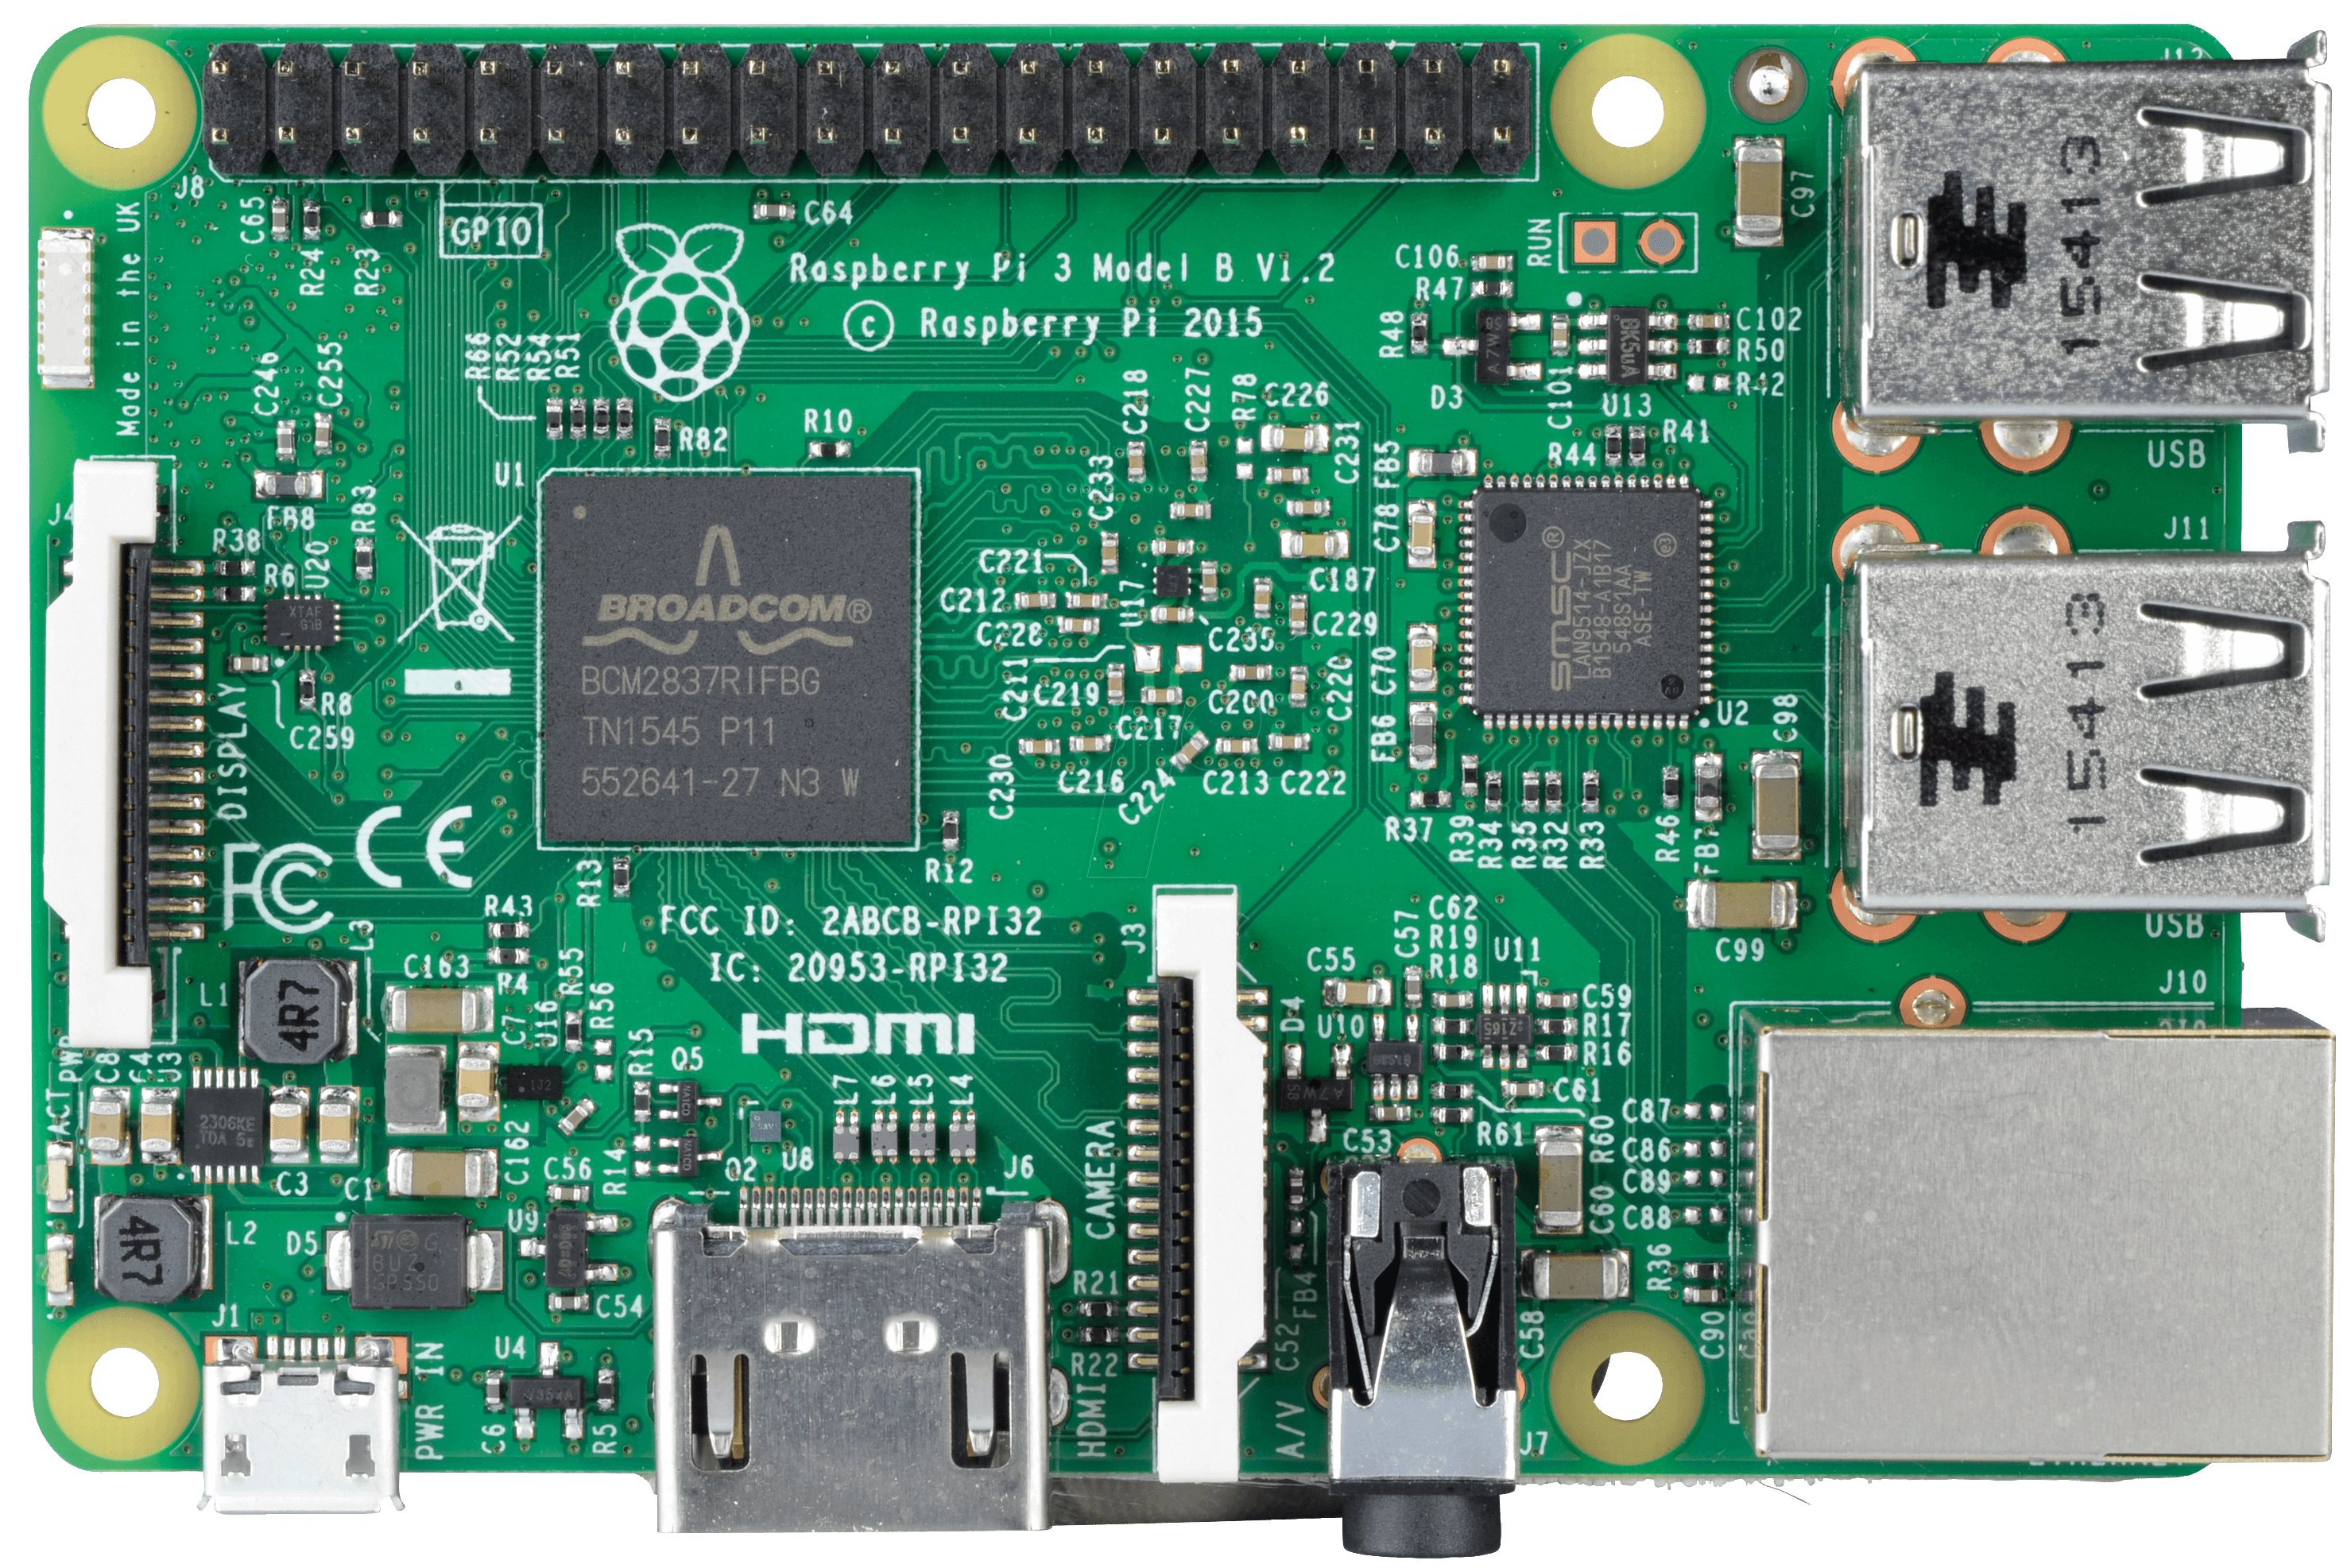
\includegraphics[scale=0.1]{Imagens/Raspberry-Pi.png}
	\centering  	
  	\captionsource{Raspberry Pi 3, Modelo B.
\label{fig:raspberry-pi}}{\cite{Xbian}}
  	
\end{figure}


\section{Sensor RFID MFRC522}

O MFRC522 mostrado na figura \ref{fig:leitor-rfid} � um leitor com poder de leitura e escritas para comunica��o sem necessidade de contato que opera em uma frequ�ncia de 13.56  MHz. O leitor se comunica com cart�es que possuem os padr�es ISO/IEC 14443 e  A/MIFARE cards. O MFRC522 permite a comunica��o atrav�s das interfaces \cite{nxp}


\begin{figure}
	\centering
  	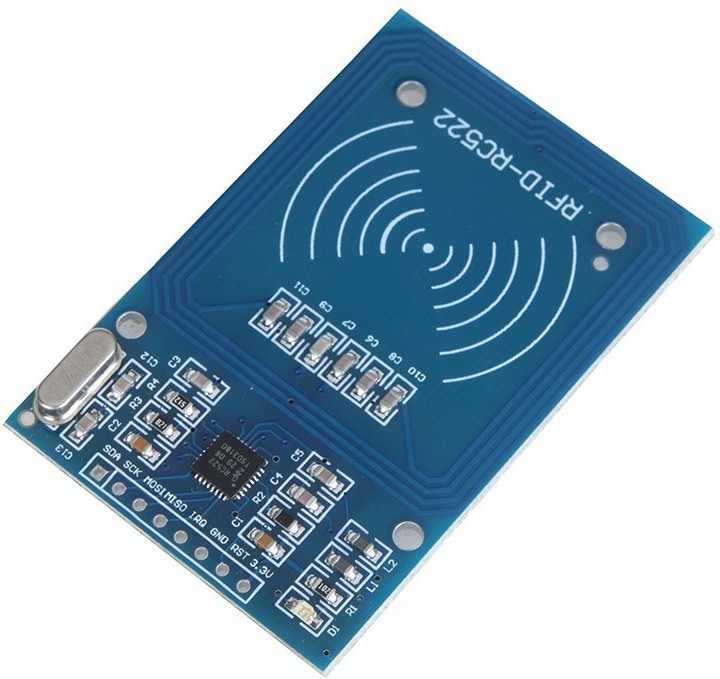
\includegraphics[scale=0.3]{Imagens/leitor-rfid-rc522.jpg}
	\centering  	
  	\captionsource{Leitor de Cart�o RFID RC522
\label{fig:leitor-rfid}}{\cite{box}}
  	
\end{figure}

Neste trabalho � utilizada a interface SPI  para a comunica��o com o leitor, e s�o utilizados cart�es e tags RFID com padr�o Mifare como as mostradas na figura \ref{fig:tag-rfid}.
 
\begin{figure}
	\centering
  	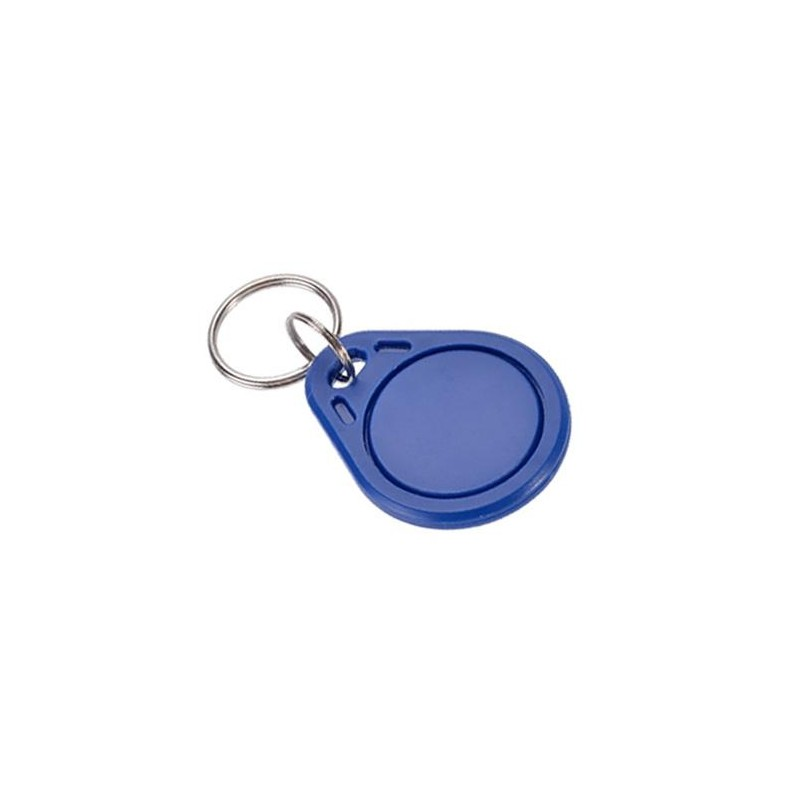
\includegraphics[scale=0.3]{Imagens/tag-rfid.jpg}
	\centering  	
  	\captionsource{Tag RFID de padr�o Mifare
\label{fig:tag-rfid}}{\cite{box}}
  	
\end{figure}

\section{Sensor PIR}
O sensor PIR (mostrado na figura \ref{fig:motion-sensor})  � utilizado comumente para a identifica��o de pessoas em um ambiente no raio de alcance do sensor. A sigla \abrv[PIR -- Passive-Infrared]{PIR} vem do ingl�s Passive-Infrared e � chamado dessa maneira por utilizar sensores piroel�tricos para detectar n�veis de radia��o infravermelha. Esse tipo de sensor n�o identifica a dist�ncia em que o corpo est� do sensor, apenas se h� algum corpo no ambiente. O alcance do sensor � de aproximadamente 6 metros e �ngulo de 110�X70� \cite{adafruit}.



 
\begin{figure}
	\centering
  	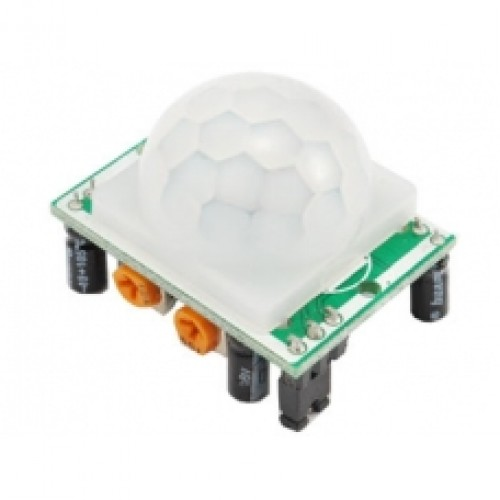
\includegraphics[scale=0.3]{Imagens/motion-sensor.jpg}
	\centering  	
  	\captionsource{Sensor PIR
\label{fig:motion-sensor}}{\cite{easy}}
  	
\end{figure}

\section{Kaa}

O Kaa � uma plataforma aberta de Middleware de IoT, que permite a constru��o de aplica��es completas desse paradigma, al�m de fornecer outras funcionalidades embutidas importantes para o desenvolvimento desse tipo de aplica��o. Segundo \citeauthor{kaaiot} (\citeyear{kaaiot})''O Kaa permite um gerenciamento de dados para os objetos conectados e a sua infraestrutura atrav�s de componentes para o servidor e SDKs para os endpoints. Os SDKs s�o embutidos nos objetos conectados e implementam troca de dados bi-direcional com o servidor.''
	O Kaa possibilita o uso de aplica��es de larga-escala em IoT, promovendo os servi�os de: comunica��o entre objetos conectados, consist�ncia de dados, seguran�a, interoperabilidade e uma conectividade a prova de erros \cite{kaaiot}.
	
\section{Pi4J}  
O Pi4J Project � um projeto idealizado para fornecer uma interface orientada a objetos mais amig�vel para programadores Java utilizarem os recursos de entrada e sa�da do Raspberry Pi. Atrav�s da abstra��o de fun��es de baixo n�vel o Pi4J proporciona essa maior facilidade de uso de E/S \cite{pi4j}.

\section{MySQL}
Segundo \citeauthor{oracle-mysql}(citeyear{oracle-mysql}) MySQL � o sistema de gerenciamento de banco de dados aberto mais popular atualmente. � mantido pela Oracle Corporation. O MySQL lida com banco de dados relacional, comumente chamado de SQL que � a sigla para Structured Query Language (Linguagem Estruturada de Consultas).
	O MySQL foi inicialmente criado para lidar grande quantidades de dados de uma forma mais r�pida que as ferramentas existentes naquela mesma �poca. Mas tamb�m acabou se popularizando no desenvolvimento de pequenas aplica��es uma vez que pode ser executado tanto em  computadores pessoais como em servidores-web, que possuem mais recursos dedicados \cite{oracle-mysql}.


\section{Spring MVC}

O Spring MVC � uma implementa��o do framework Spring para aplica��es web baseado no modelo arquitetural model-view-controller. O Framework Spring � uma plataforma Java que permite o desenvolvimento de aplica��es com suporte  focado para a infraestrutura da aplica��o, o framework auxilia permitindo um desacoplamento das diferentes partes da aplica��o. O modelo MVC est� focado na divis�o das camadas  de uma aplica��o em visualiza��o(\textit{view}) (que s�o os elementos que o usu�rio interage), modelo(\textit{model}) que � a representa��o em c�digo dos objetos do mundo real e controles(\textit{controllers}), que faz a l�gica da aplica��o e permite a comunica��o dos dois anteriores. O Spring MVC permite o desacoplamento das camadas que comp�em uma aplica��o wev e oferece as funcionalidades do framework Spring \cite{johnson}.

	
	% Capitulo 3: Terceiro cap�tulo (arquivo Includes/Capitulo3.tex)
	% Cap�tulo 3
\chapter{Trabalhos Relacionados}

\section{Solu��es para pr�dios inteligentes}
\subsection{A Smart Room Scheduling and Management System with Utilization Control and Ad-hoc Support Based on Real-Time Occupancy Detection}

Previamente ao desenvolvimento da aplica��o Roomie foram pesquisados outros trabalhos cient�ficos e softwares que possu�am foco no tema de controle de espa�os f�sicos em pr�dios. Essas refer�ncias possibilitaram a aquisi��o de um maior conhecimento sobre o problema e o desenvolvimento de uma aplica��o que tentasse resolver problemas que as solu��es anteriores n�o resolviam. 

O principal objetivo do trabalho de \citeauthor{tran} (\citeyear{tran}) � a constru��o de um sistema inteligente de reserva de salas que endere�a o problema de subutiliza��o de salas de reuni�o. Essa subutiliza��o segundo o autor � causada principalmente por reuni�es que n�o acontecem mas possuem reservas no sistema e por sistemas que n�o suportam disponibilidade em tempo real de novas reservas. A solu��o proposta para combater o problema reportado � atrav�s de uma aplica��o que permite a ci�ncia sobre status de ocupa��o das salas em tempo-real e que promove a integra��o dessa informa��o com sistema de reserva.  

O sistema descrito no trabalho � composto por sensores de movimento (PIR) , cada sala possui um sensor conectado a um sistema embarcado que por sua vez possui uma uma conex�o ethernet. Os sensores s�o utilizados para detec��o de presen�a e os sinais captados s�o enviados via protocolo UDP(User Datagram Protocol) pelo sistema embarcado para um servidor que controla as reservas e que disponibiliza uma interface para os usu�rios gerenciarem suas reservas. A organiza��o do sistema � ilustrada na figura \ref{fig:isense}.

\begin{figure}
	\centering
  	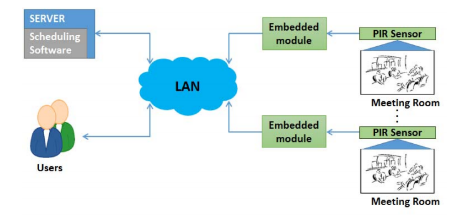
\includegraphics[scale=0.8]{Imagens/isense.png}
	\centering  	
  	\captionsource{Vis�o Geral do sistema
\label{fig:isense}}{\cite{tran}}
  	
\end{figure}
Principais funcionalidades do sistema:
\begin{itemize}

\item Cancelamento de reserva autom�tico por n�o detec��o de presen�a;
\item Gerenciamento de reservas em uma Interface Web pr�pria;
\item Fornecimento da informa��o em tempo real sobre a disponibilidade das salas; 
\end{itemize}

%\begin{enumerate}
%	\item ter um extremo cuidado durante a reda��o do texto, principalmente com rela��o �s regras gramaticais e ortogr�ficas da l�ngua; geralmente todo o texto � escrito na forma impessoal do verbo, n�o se utilizando, portanto, de termos em primeira pessoa, seja do plural ou do singular.
%\end{enumerate}

\subsection{iSense: A Wireless Sensor Network Based Conference Room Management System}
O trabalho de  \citeauthor{padma} (\citeyear{padma})  �  em um sistema de reservas de salas que permite a detec��o de presen�a e status dos aparelhos eletr�nicos utilizados na sala. O foco do estudo � o melhor uso dos espa�os atrav�s de espa�os com maior consci�ncia sobre sua ocupa��o e sobre a  utiliza��o de aparelhos eletr�nicos na sala. 
	O sistema descrito no trabalho (chamado de iSense) � composto de um microcontrolador com sensores (sensor de presen�a, temperatura e luminosidade) conectados a ele, um transceptor sem fio, um gateway, uma aplica��o de controle e um banco de registro de dados.  Todos os dados coletados dos sensores s�o enviados para um gateway conectado a um computador e interpretados por uma aplica��o de controle. Os sensores s�o utilizados usados para detec��o de pessoas (microfone e PIR sensor) e os outros sensores (luz e temperatura) s�o utilizados para a medi��o do consumo de energia. O funcionamento do iSense segue da seguinte maneira:

\begin{enumerate}

\item Usu�rio solicita atrav�s do iSense uma reserva;
\item iSense checa se a sala no hor�rio estabelecido est� livre no MS Outlook, caso esteja confirma a reserva sen�o fornece a  op��o do usu�rio entrar em uma fila para a reserva espec�fica;
\item O iSense monitora o uso das salas atrav�s dos sensores, caso uma sala for indicada n�o ocupada por 5 minutos ap�s o tempo inicial, o dono da reserva recebe uma mensagem requisitando o cancelamento da reserva.
\item Caso o usu�rio cancele a reserva, a pr�xima reserva que estava na lista de espera � alocada para o espa�o da reserva cancelada.

\end{enumerate}

O iSense foi utilizado no campus da empresa que os autores trabalhavam e obtiveram como resultado final, um aumento de 27% de uso das salas de reuni�o e uma redu��o de 13% em energia el�trica. 			
Principais funcionalidades do iSense:
\begin{itemize}
\item Sistema de fila para reservas;
\item Conex�o com Microsoft Outlook para efetuar reservas;
\item Disponibiliza��o das informa��es sobre os aparelhos eletr�nicos ligados na sala (ar-condicionado e luzes).
\item Sistema de detec��o de presen�a;
\end{itemize}

%\begin{enumerate}
%	\item ter um extremo cuidado durante a reda��o do texto, principalmente com rela��o �s regras gramaticais e ortogr�ficas da l�ngua; geralmente todo o texto � escrito na forma impessoal do verbo, n�o se utilizando, portanto, de termos em primeira pessoa, seja do plural ou do singular.
%\end{enumerate}

\section{Comparativo entre solu��es}

Na tabela \ref{tab:TabelaComparativa} � feita uma compara��o entre as solu��es encontradas na literatura descritas na se��o 3.1, baseado nas funcionalidades que os sistemas disponibilizam. E abaixo segue uma legenda para a tabela \ref{tab:TabelaComparativa}.


\begin{enumerate}

\item A Smart Room Scheduling and Management System with Utilization Control and Ad-hoc Support Based on Real-Time Occupancy Detection
\item iSense: A Wireless Sensor Network Based Conference Room Management System
\end{enumerate}

\begin{table}[htb]
	% T�tulo de tabelas sempre aparecem antes da tabela
	\textsf{\caption{ Comparativo de solu��es de reserva de salas}}
	\center
	\begin{center}
	
		\begin{tabular}{|l|c|r|}
			\hline
			\textbf{Funcionalidade}&\textbf{1}&\textbf{2}\\
			\hline			
			Detec��o de Presen�a& Sim&Sim\\
			Status de ocupa��o de salas em tempo real&Sim&N�o\\
			Autentica��o na entrada da sala&N�o&N�o\\	
			Sistema de Gerenciamento de Reservas Pr�prio&Sim&N�o\\					
			Simplicidade no acoplamento de novos sensores& N�o&N�o\\
			Status dos equipment eletr�nicos& N�o&Sim\\
			Cancelamento autom�tico de reservas por Inatividade& Sim&N�o\\
			\hline				 		 		
		\end{tabular}
	\end{center}
	\label{tab:TabelaComparativa}
\end{table}

	
	% Capitulo 4: Quarto cap�tulo (arquivo Includes/Capitulo4.tex)
	% Cap�tulo 4
s\chapter{Rommie: uma aplica��o para pr�dios inteligentes}

Poucos exemplos de  aplica��es que lidam com o tema de reserva de espa�os em pr�dios foram encontrados na literatura, os exemplos mais pr�ximos encontrados foram os trabalhos citados na se��o 3. Esses trabalhos possuem focos diferentes e atendem a alguns requisitos similares como exemplificado no quadro 01, mas ambos n�o suportam autentica��o para o uso da salas e n�o d�o suporte a uma maneira simples e f�cil de acoplamento de novos sensores e dispositivos.  Em consequ�ncia  dessas funcionalidades n�o serem encontradas nas solu��es anteriores, foi realizado o desenvolvimento da aplica��o Roomie, que foi focada principalmente na incorpora��o do IoT. Nas pr�ximas se��es ser� descrito a aplica��o Roomie em termos de arquitetura, requisitos e desenvolvimento das aplica��es.


\section{Concep��o e Design da Aplica��o}
\subsection{Arquitetura da Aplica��o}

O sistema Roomie � composto por 3 diferentes aplica��es. Cada uma com seu prop�sito especif�co. Sendo a primeira uma aplica��o Web que tem como principal objetivo fornecer uma interface amig�vel para os usu�rios gerenciarem suas reservas; a segunda � a aplica��o que roda no Raspberry Pi que � focada em trazer informa��es vindas de sensores para compor o sistema, e a terceira a chamada  aplica��o de controle que tem como principal objetivo ajudar na coordena��o de todo o sistema Roomie. A arquitetura � dividida na estrutura apresentada na Figura \ref{fig:arq}. 

\begin{figure}[htb]
	\centering
  	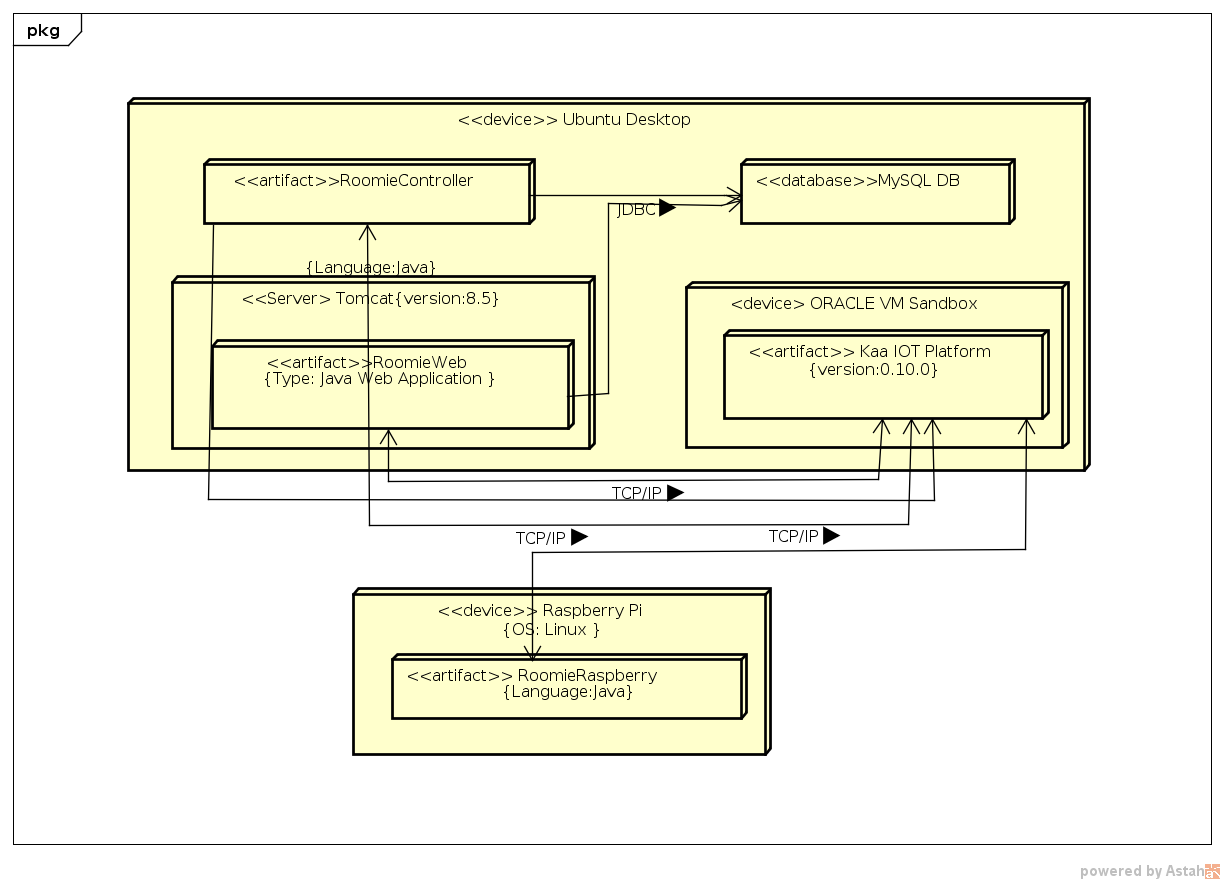
\includegraphics[scale=0.5]{Imagens/DiagramaArquitetura.png}
	\centering  	
  	\captionsource{ Diagrama de Implementa��o
\label{fig:arq}}{Pr�prio Autor}
  	
\end{figure}
Abaixo segue uma descri��o detalhada da arquitetura, onde os n�meros romanos representam os dispositivos e as letras os softwares ou aplica��es que rodam nesses dispositivos.
\begin{enumerate}
\item Desktop Ubuntu
\begin{enumerate}
\item RoomieController: Aplica��o de controle desenvolvida na linguagem Java, tem como principal objetivo fazer o controle de disparos de eventos para as outras aplica��es que est�o rodando em outros dispositivos e o controle da aplica��o no geral.
\item RoomieWeb: Aplica��o Web em Spring MVC que permite o usu�rio gerenciar suas reservas em uma interface amig�vel. 
\item Plataforma Kaa IOT: � o \textit{middleware} de IoT respons�vel pela conex�o das aplica��es distintas, essa comunica��o � baseada atrav�s do uso de eventos.
\item Banco de Dados MySQL: Banco de dados local respons�vel pelo armazenamento de dados de usu�rio e das reservas. 
\end{enumerate}
\begin{enumerate}
\item Desktop Ubuntu
\begin{enumerate}
	\item RoomieRaspberry: aplica��o Java respons�vel pela capta��o e interpreta��o dos dados coletados pelos sensores e envio por meio de eventos para o Kaa.
	\end{enumerate}
\end{enumerate}
\end{enumerate}
A comunica��o entre as aplica��es e o Middleware Kaa � realizada atrav�s do envio de eventos, que s�o disparadas pelas diferentes aplica��es enviadas para o Kaa e depois para as aplica��es de destino atrav�s do  protocolo TCP/IP. Enquanto que a comunica��o das aplica��es com o banco local � realizada atrav�s da API do Java de comunica��o com o banco de dados, o JDBC.


\subsection{Requisitos da Aplica��o}

Um software � constru�do para resolver um problema ou v�rios problemas levantados por alguma organiza��o ou indiv�duo, no entanto essa � uma vis�o bastante ampla do que o sistema precisa realizar, por isso � preciso descrever mais detalhadamente as funcionalidades e comportamento esperados. Uma descri��o exata do que o sistema deve fazer pode ser expressada atrav�s de requisitos, requisitos s�o as fun��es e restri��es da aplica��o. Os requisitos do Roomie ser�o divididos em requisitos funcionais e n�o-funcionais., enquanto o outro � utilizado para descrever caracter�sticas mais gen�ricas do sistema e normalmente n�o de funcionalidades \cite{sommerville}.
\subsubsection{Requisitos Funcionais}
Os requisitos funcionais (RF) s�o utilizados para descrever as funcionalidades ou servi�os promovidos pelo sistema \cite{sommerville}. Na tabela \ref{tab:TabelaRequisitos}, s�o especificados os requisitos da aplica��o Roomie.

\begin{table}
\begin{center}
\begin{tabular}{ | c | c | c |}
\hline
\thead{C�digo} & \thead{Nome} & \thead{A Third \\ Head} \\
\hline
RF01   & Efetuar Login& \makecell{O usu�rio deve efetuar login \\ no RoomieWeb para gerenciar suas reservas } \\ \hline
RF02   & Cadastrar Reservas           & \makecell{Permite o usu�rio cadastrar novas reservas \\ RoomieWeb.}\\ \hline                                                                
RF03   & Excluir Reservas             & \makecell{Permite o usu�rio excluir suas reservas no \\ RoomieWeb.}\\ \hline                                                                                
RF04   & Visualizar Reservas          & \makecell{Permite o usu�rio visualizar suas reservas no \\ RoomieWeb}\\ \hline                                                                                                                                                              
RF05   & Acessar sala com cart�o RFID & 
\makecell{O Acesso a sala reservada deve ser feito\\ apenas aos usu�rios cadastrados na reserva\\
, atrav�s da utiliza��o do cart�o RFID cadastrado}
\\ \hline
\end{tabular}
\end{center}
\caption{Lista de requisitos funcionais}
\label{tab:TabelaRequisitos}
\end{table}

\subsubsection{Modelagem de Casos de Uso}

Uma forma de representar esses requisitos e os personagens que participam nele � atrav�s de um diagrama de casos de uso, esse modelo tem como principal finalidade modelar as funcionalidades do sistema \cite{bezerra}. Na figura \ref{fig:usecase} tem-se o  diagrama de casos de uso para o sistema Roomie. 

As descri��es completas dos casos de uso da figura \ref{fig:usecase} se encontram no Ap�ndice A. A tabela \ref{tab:TabelaAtores} cont�m a descri��o dos atores (qualquer elemento externo que interaja com o sistema).


\begin{figure}[htb]
	\centering
  	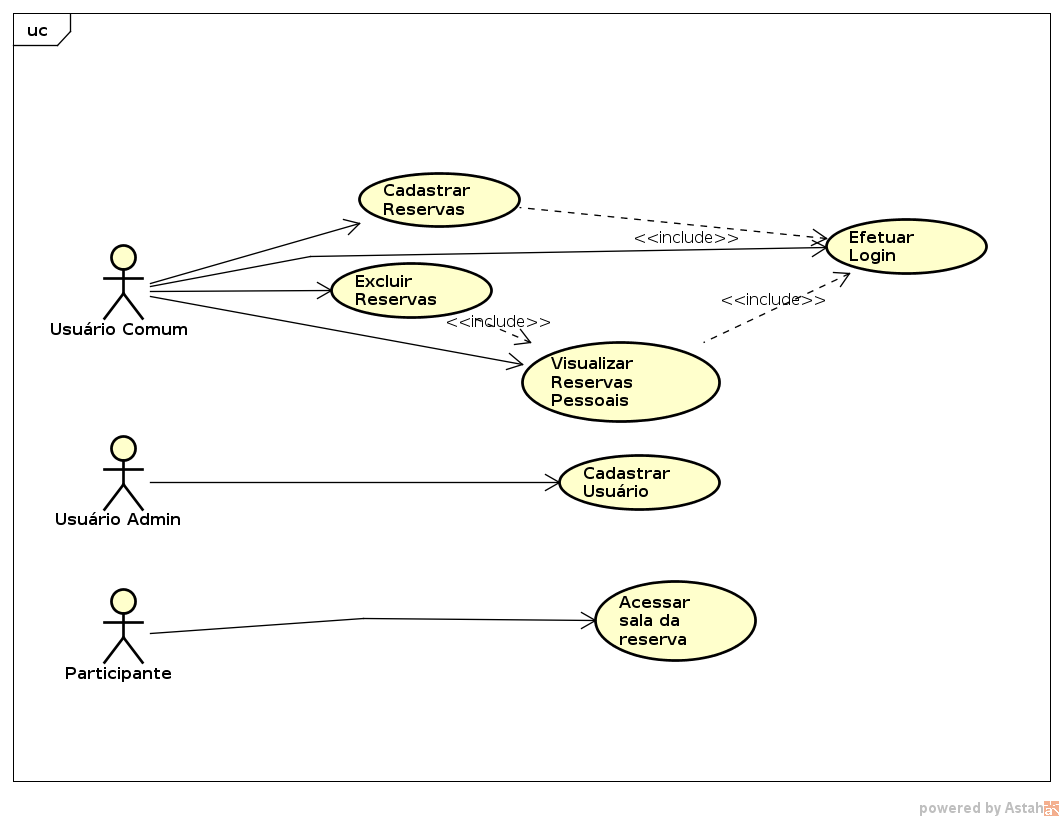
\includegraphics[scale=0.5]{Imagens/UseCase.png}
	\centering  	
  	\captionsource{ Diagrama de Casos de Uso
\label{fig:usecase}}{Pr�prio Autor}
  	
\end{figure}

\begin{table}
\begin{center}
\begin{tabular}{ | c | c | c |}
\hline
\thead{Ator}&\thead{Descri��o}\\ \hline
Usu�rio Comum&\makecell{Usu�rio que est� logado na\\ aplica��o RoomieWeb.}\\ \hline
Usu�rio Admin&\makecell{Usu�rio que possui o acesso ao\\ RoomieRaspberry.}\\ \hline
Participante&\makecell{� o usu�rio que possui \\cadastro no banco de dados, mas n�o \\ necessariamente reservou uma sala. Mas est� inclu�do \\ na reserva como participante de uma reuni�o.}\\ \hline
\end{tabular}
\end{center}
\caption{Atores}
\label{tab:TabelaAtores}
\end{table}

\subsubsection{Requisitos N�o Funcionais}

Os requisitos n�o funcionais (RNF)  por sua vez s�o utilizados para descrever caracter�sticas mais gen�ricas do sistema e normalmente n�o de funcionalidades espec�ficas \cite{sommerville}. A tabela \ref{tab:TabelaRNF}, s�o especificados os requisitos n�o funcionais da aplica��o Roomie.



\begin{table}
\begin{center}
\begin{tabular}{ | c | c | c |}

\hline
\thead{C�digo}\thead{Nome}&\thead{Descri��o}\\ \hline
RNF01&Tempo de Resposta&
\makecell{O tempo de resposta\\ das aplica��es conectadas devem ser \\
near real-time.}\\ \hline
RNF02&Seguran�a na
Aplica��o Web&\makecell{O sistema deve permitir apenas\\ aos usu�rios logados permiss�o para gerenciar\\ reservas.}\\ \hline"
RNF03&Interface&\makecell{As aplica��es com interfaces\\ com o usu�rio devem ser claras e objetivas.}\\ \hline
RNF04&Armazenamento de Senhas&
\makecell{Apenas a senha no formato SHA256 ser�\\ armazenada no banco de\\ dados;}\\ \hline
RF05&Acessar sala com cart�o RFID&\makecell{O Acesso a\\ sala reservada deve ser \\eito apenas aos usu�rios\\ cadastrados na reserva,\\ atrav�s da utiliza��o do \\cart�o RFID cadastrado.}\\ \hline
\end{tabular}
\end{center}
\caption{ Lista de requisitos n�o funcionais}
\label{tab:TabelaRNF}
\end{table}

\subsection{Diagrama de Classes}
Diagrama de classes s�o utilizados para representar o aspecto estrutural e est�tico do sistema. Est�tico por n�o descrever o comportamento dos objetos do sistema ao longo do tempo e estrutural por focar no relacionamento entre as partes do sistema \cite{bezerra}. Na Figura \ref{fig:classesRoomie} � mostrado o Diagrama de classes do sistema Roomie, focado em um n�vel geral das diferentes aplica��es e os pacotes que comp�em as aplica��es. Na se��o 4.2 ser�o inclu�dos outros diagramas de classes com mais detalhes estruturais das diferentes aplica��es.

\begin{figure}[htb]
	\centering
  	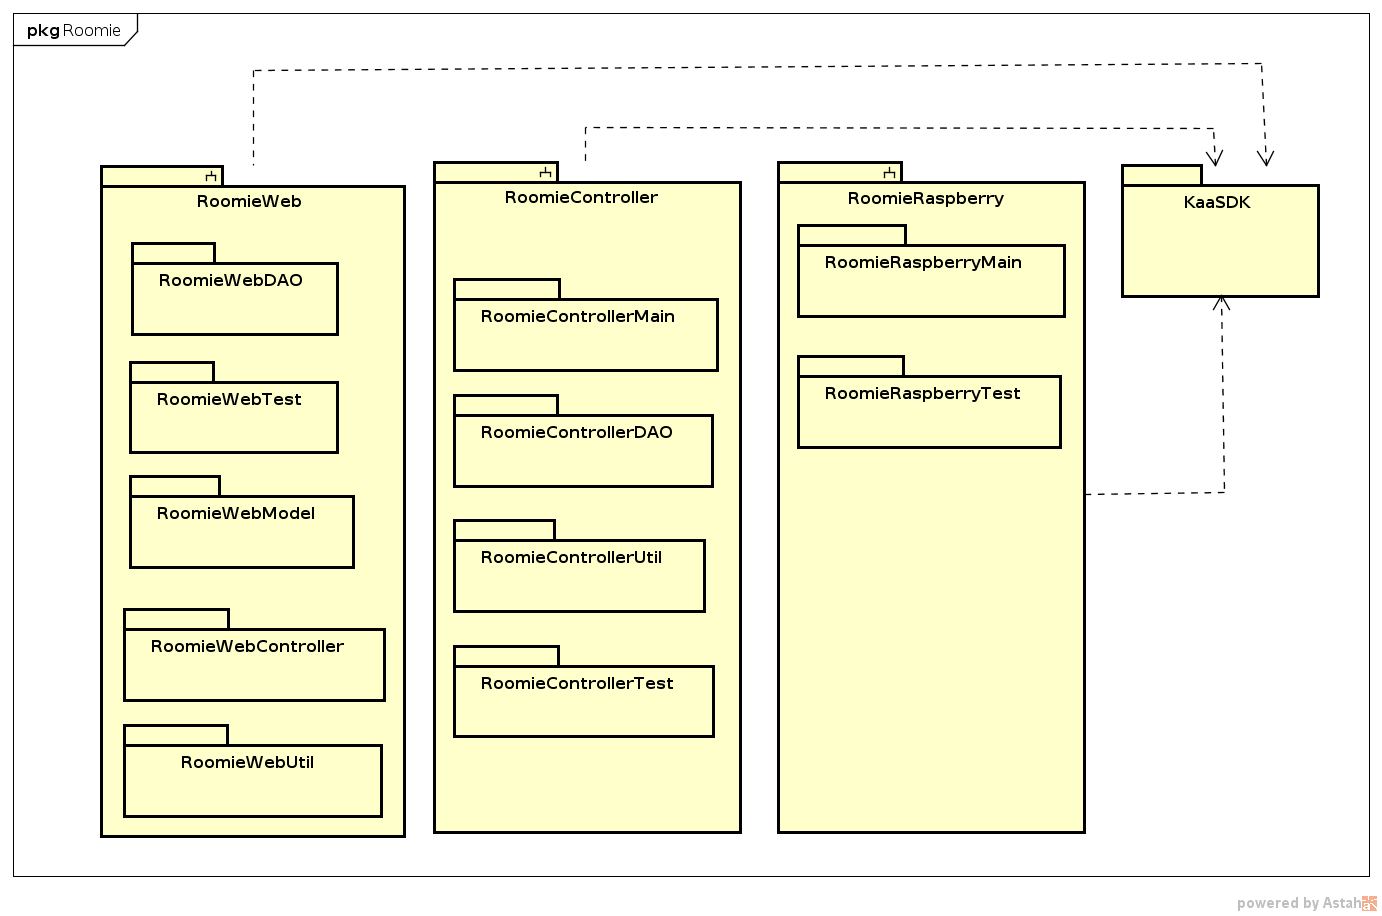
\includegraphics[scale=0.5]{Imagens/Overview.png}
	\centering  	
  	\captionsource{ Diagrama de Classes Roomie
\label{fig:classesRoomie}}{Pr�prio Autor}
  	
\end{figure}

\subsection{Modelo de Processo de Neg�cio}
Nesta se��o � utilizado o modelo de processo de neg�cio ou mais conhecido como BPM (\textit{Business Process Model}) para mostrar o comportamento e procedimentos mais importantes dentro dos sistemas Roomie. Esse tipo de diagrama consegue capturar bem fluxos de sequ�ncias e mensagens entre diferentes processos, algo que � bastante importante na aplica��o Roomie, uma vez que os diferentes sistemas se comunicam constantemente atrav�s de envio de mensagens.O modelo da figura \ref{fig:bpmn} descreve o fluxo de uma reserva realizado pela aplica��o Roomie.

\begin{figure}[htb]
	\centering
  	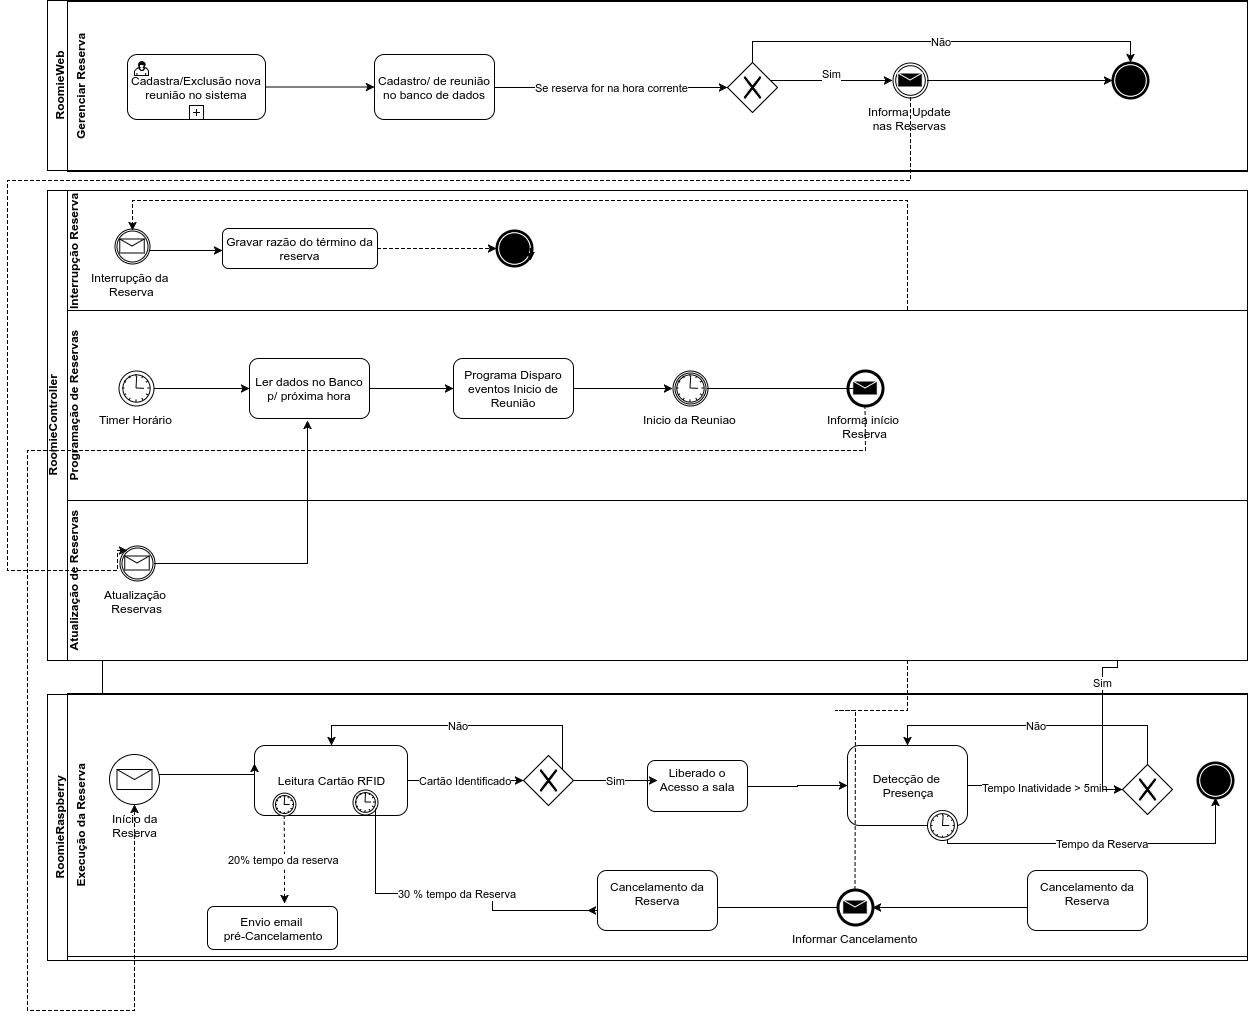
\includegraphics[scale=0.5,angle=90,origin=c]{Imagens/BPMN.png}
	\centering  	
  	\captionsource{BPM de Fluxo de reserva do Sistema Roomie
\label{fig:bpmn}}{Pr�prio Autor}
  	
\end{figure}

Descri��o do BPM     

\begin{enumerate}
\item RoomieWeb
\begin{enumerate}
\item Gerenciar Reserva: Inicia quando o usu�rio modifica ou cria uma nova reserva e, logo ap�s ocorre a grava��o da mudan�a no banco de dados, caso essa reserva aconte�a na hora corrente � enviada uma mensagem de atualiza��o para o RoomieController, caso a reserva n�o aconte�a na hora corrente o fluxo se encerra na atualiza��o do banco.
\end{enumerate}
\item RoomieController: como descrito anteriormente o RoomieController tem como principal funcionalidade coordenar o sistema como um geral.
Como mostrado no BPM existem 3 fluxos que podem acontecer nessa inst�ncia do sistema:

\begin{enumerate}
 
\item Interrup��o de reserva: inicia quando a um recebimento de uma mensagem informando que uma reserva foi interrompida, a mensagem � enviada pelo Roomie Raspberry. Ap�s isso ocorre uma grava��o do cancelamento da reuni�o no banco dados  e o fluxo termina.
\item Programa��o de reservas: de hora em hora um tarefa de programa��o para recuperar as reservas da hora seguinte � executada e s�o agendados os envio de mensagens de in�cio das reservas para serem disparadas no hor�rio da reserva. Quando o hor�rio da reserva chega o sistema envia uma mensagem de in�cio da reserva para o Roomie Raspberry e o fluxo se encerra.
\item Atualiza��o de Reservas: Quando alguma reserva da hora corrente � modificado � recebida uma mensagem indicando atualiza��o na reserva, logo ap�s isso s�o feitos os passos de atualizar as reservas que foram recuperadas para a hora corrente.

\end{enumerate}
\item RoomieRaspberry
\begin{enumerate}
\item Caso o cart�o fornecido seja igual o de algum participante da reserva, o acesso a sala � liberado.Logo ap�s o sistema entra no modo de detec��o de presen�a, caso a sala fique com inatividade por mais de 5 minutos � enviada uma mensagem para o cancelamento da reserva. Caso n�o for registrado inatividade o sistema continua em detec��o da presen�a at� o fim do tempo da reserva e o fluxo finaliza.			
\item Caso contr�rio o sistema  continua em modo de leitura at� o que o cart�o v�lido seja fornecido, caso se passe 20\% do tempo da reserva � enviando um email alertando o usu�rio do  poss�vvel cancelamento. Caso chegue a marca de 30\% do tempo total da reserva e nenhum cart�o seja identificado a reserva � cancelada e � enviada uma mensagem para o cancelamento da reuni�o para o RoomieController.

\end{enumerate}

\end{enumerate}

\section{Implementa��o e Testes da Aplica��o}

\subsection{Desenvolvimento da aplica��o no Middleware Kaa}

Para trazer a aplica��o de reservas Roomie para o mundo de IoT foi utilizado o middleware Kaa, o Kaa possibilita a troca de mensagens entre as aplica��es de maneira simples e com pequeno esfor�o.
	A escolha do Kaa como middleware partiu pelo fato de ser uma plataforma de c�digo-aberto, que � independente de plataforma e por ser atualmente estar sendo atualizada constantemente. Propiciando um espa�o mais seguro e simples para o desenvolvimento da aplica��o.
\subsubsection{Configura��o da Instala��o do Kaa}

Para a implementa��o do Roomie, o Kaa foi instalado em uma m�quina virtual, a Oracle VM Virtual Box - 5.1.2, com 2GB reservados para a m�quina virtual e com uso de 2 processadores. 

\subsubsection{Vis�o Geral da Arquitetura e funcionamento do Kaa}

A arquitetura do Kaa segundo \cite{cybervision} � formada basicamente por tr�s partes distintas:
\begin{itemize}

\item Servidor Kaa : � a parte back-end da plataforma, � respons�vel pelo gerenciamento dos elementos que s�o acoplados a ferramenta como as aplica��es, dispositivos e elementos internos.
\item Extens�es Kaa: s�o softwares independentes do Kaa, que ajudam o Kaa em fun��es espec�ficas. Exemplos dessas extens�es como mostrado na figura 08 � o Zookeeper Apache e  bancos de dados SQL e NoSQL.
\item \textit{Endpoints SDKs}:  Os endpoints SDKs s�o bibliotecas instaladas nos dispositivos a serem conectados no Kaa. Esse sdk permite uma comunica��o f�cil e padronizada com o Kaa atrav�s de uma API. 


\end{itemize}


\begin{figure}[htb]
	\centering
  	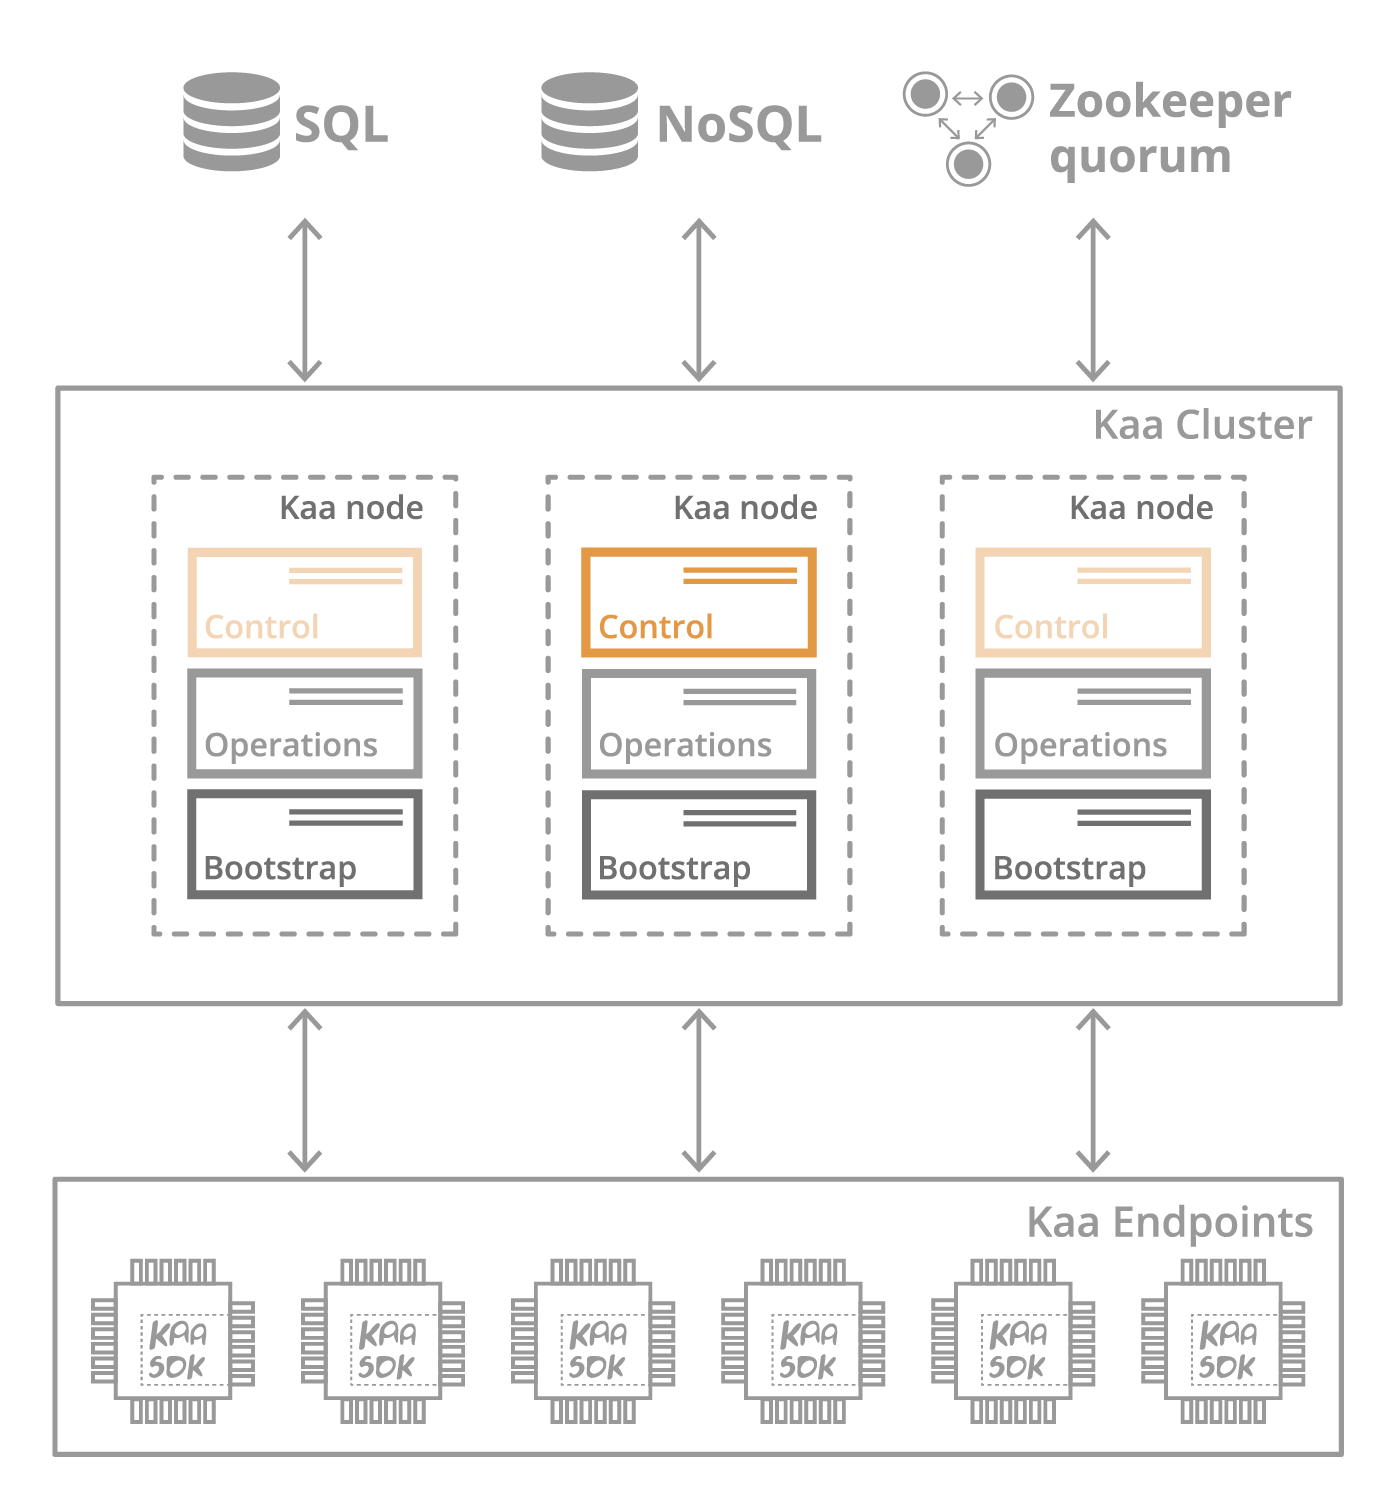
\includegraphics[scale=0.2]{Imagens/kaa-arq.png}
	\centering  	
  	\captionsource{Arquitetura Kaa
\label{fig:kaa-arq}}{\cite{cybervision-arq}}
  	
\end{figure}

Existem dois tipos de mensagens de comunica��o entre o servidor kaa e os \textit{endpoints sdks}, s�o as notifica��es e os eventos. As notifica��es s�o utilizadas para envio de mensagens do servidor Kaa para os endpoints que est�o cadastrados no mesmo t�pico. Enquanto que os eventos s�o utilizados para o envio de informa��es de \textit{endpoints} para outros \textit{endpoints}, e esse envio sendo gerenciado pelo servidor do Kaa. Na aplica��o Roomie utilizamos apenas eventos como meio de comunica��o dos endpoints.

\subsubsection{Eventos} 
A gera��o de eventos atrav�s da plataforma Kaa s�o suportados de maneira quase que tempo-real, os eventos s�o gerados por endpoints  gerados pelo mesmo usu�rios tratados e enviados pelo kaa para os endpoints que est�o cadastrados para o recebimento do evento espec�fico. Os dados enviados nos eventos s�o configur�veis no pr�prio Kaa, cada evento possuindo esquema diferente para classe que representa um evento \cite{cybervision-events}.
	Cada evento possui uma classe de evento associada a ele, n�o podendo assim existir dois eventos com a mesma classe. Classes de evento (EC) s�o organizadas em fam�lias de classes de eventos (ECF). Cada \textit{endpoint} cadastra para o recebimento de uma classe de fam�lia, se o \textit{endpoint} recebe um evento de uma fam�lia espec�fica deve ser configurado para receber todos os eventos da fam�lia espec�fica. O envio de eventos pode ser feito para um \textit{endpoint} espec�fico (unicast) ou para todos os \textit{endpoints} cadastrados para o recebimento para aquele evento (multicast) \cite{cybervision-events}.\\
	\textbf{Classificando \textit{endpoints} segundo a ECF}
	Os endpoints podem enviar, receber e enviar/receber eventos de uma ECF. Para distinguir os pap�is do endpoints na configura��o do endpoint podemos classificar \textit{endpoint} segundo a uma ECF  de tr�s maneiras:
\begin{itemize}
\item source: apenas envia eventos mas n�o os recebe;
\item sink : apenas recebe eventos;
\item both: recebe e envia evento da ECF espec�fica;\\

\end{itemize}	
\textbf{
Eventos no Roomie}

Para realizar a trocas de informa��es entre as diferentes aplica��es Roomie  s�o utilizado os eventos do Kaa. Na Figura \ref{fig:events} � mostrado um diagrama ilustrando os eventos utilizados no Roomie. Na tabela \ref{tab:TabelaEventos01} se encontra descri��o de todos os eventos utilizados pelo sistema Roomie. E na tabela \ref{tab:TabelaEventos02} uma descri��o eventos e dos dados que s�o enviados por cada evento, a tabela \ref{tab:TabelaEventos03} � usado como apoio para a descri��o de objetos.

\begin{figure}[htb]
	\centering
  	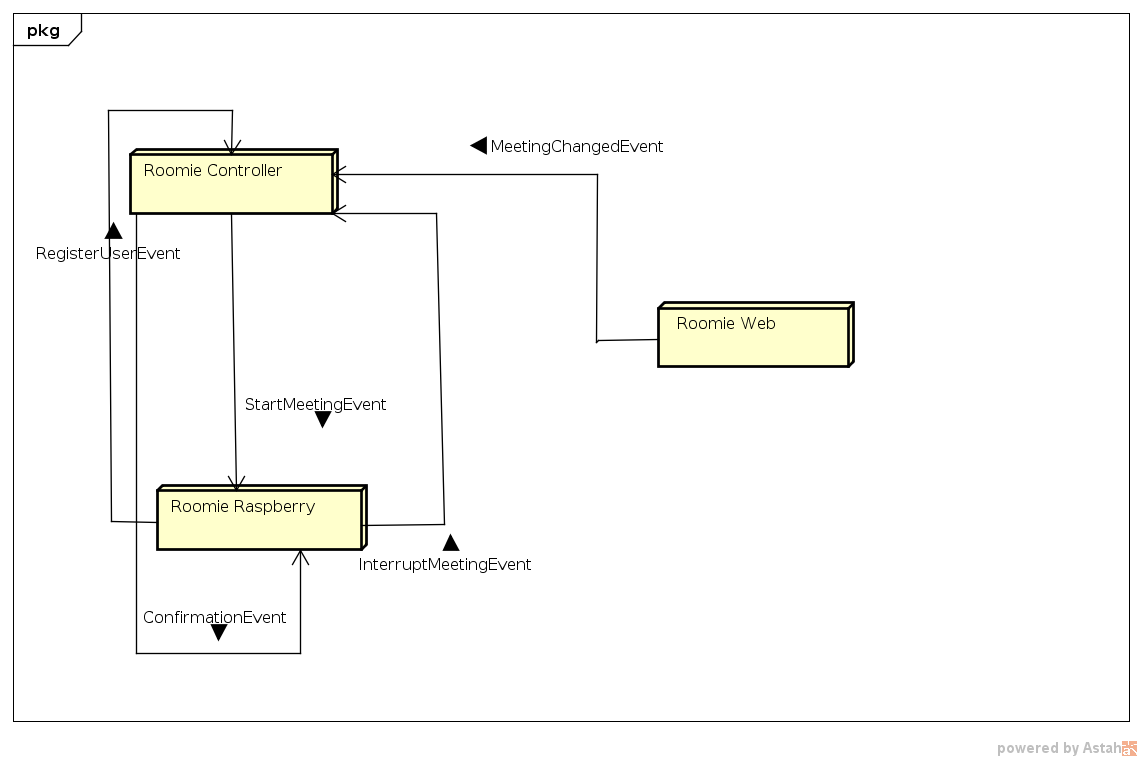
\includegraphics[scale=0.5]{Imagens/events.png}
	\centering  	
  	\captionsource{Arquitetura Kaa
\label{fig:events}}{Pr�prio Autor}
  	
\end{figure}

\begin{table}
\begin{center}
\begin{tabular}{ | c | c | c |}
\hline

\thead{Fam�lia de Eventos}&\thead{Evento}&\thead{Descri��o}\\ \hline
RegisterUserECF&RegisterUserEvent&\makecell{Evento de registro de novo usu�rio}\\ \hline
ConfirmationEventECF&ConfirmationEvent&\makecell{Evento de confirma��o \\ de cadastro de usu�rio}\\ \hline
StartMeetingECF&StartMeetingEvent&
\makecell{Sinaliza o in�cio de uma \\ reuni�o enviando \\as informa��es da reuni�o}\\ \hline
InterruptingMeetingECF&InterruptMeetingEvent&
\makecell{Evento de Cancelamento de Reserva}\\ \hline
MeetingChangedECF&MeetingChangedEvent&
\makecell{Sinaliza que uma reserva\\ na hora atual foi\\ modificada}\\ \hline
\end{tabular}
\end{center}
\caption{ Lista de requisitos n�o funcionais}
\label{tab:TabelaEventos01}
\end{table}

\begin{table}
\begin{center}
\begin{tabular}{ | c | c | c | c |}
\hline
	\thead{Evento}&\thead{Dados enviados}&\thead{Quem envia}&\thead{Quem recebe}\\ \hline
	RegisterUserEvent&user: User
user:User&\makecell{RoomieRaspberry}&\makecell{RoomieController}\\ \hline
	ConfirmationEvent&
		\makecell{status:String\\email:String\\
		isRegistered:Boolean}
         &\makecell{RoomieController}&
         \makecell{RoomieRaspberry}\\  	    \hline 
    StartMeetingEvent&meeting:Meeting&
    \makecell{RoomieController}&\makecell{RoomieRaspberry}\\ 	\hline
	InterruptMeetingEvent
	&\makecell{meetingId:Integer\\interruptReason:String}    		    		  &\makecell{RoomieRaspberry}
	&\makecell{RoomieController}\\ \hline MeetingChangedEvent&meetingId:Integer
&\makecell{RoomieWeb}&\makecell{RoomieController}\\				             	\hline
\end{tabular}
\end{center}
\caption{ Descri��o detalhada dos eventos}
\label{tab:TabelaEventos02}
\end{table}



\begin{table}
\begin{center}
\begin{tabular}{ | c | c |}
\hline
	\thead{Objeto}&\thead{Descri��o dos campos}\\ \hline
User&\makecell{userName: String \\email: String\\
hashedPassword: String\\
isOwner:boolean\\
rfidCode: String;}\\ \hline"
Meeting&\makecell{users: Array Users
\\startTime:String
\\endTime:String
\\meetingName:String
\\meetingId:Integer
\\roomLocation:String
\\roomId:Integer
\\roomName:String}\\ \hline

\end{tabular}
\end{center}
\caption{Descri��o dos objetos suporte}
\label{tab:TabelaEventos03}
\end{table}

\subsubsection{C�digos Conex�o Kaa - Java }
Nesta se��o s�o apresentados c�digos b�sicos utilizados para a conex�o com a plataforma Kaa.\\
\textbf{C�digo de Inicializa��o do Kaa  
}
No trecho da figura \ref{fig:start-event}, um cliente Kaa � inicializado, e s�o definidos comportamentos para serem executados depois da inicializa��o e para quando o Kaa for pausado. Como as chamadas do Kaa s�o ass�ncronas, ou seja, o c�digo continua a ser executado e n�o espera o fim da execu��o da chamada, � utilizado um mecanismo para pausar a thread principal at� a chamada ser finalizada e o fim dela ser sinalizado.


\begin{figure}[htb]
	\centering
  	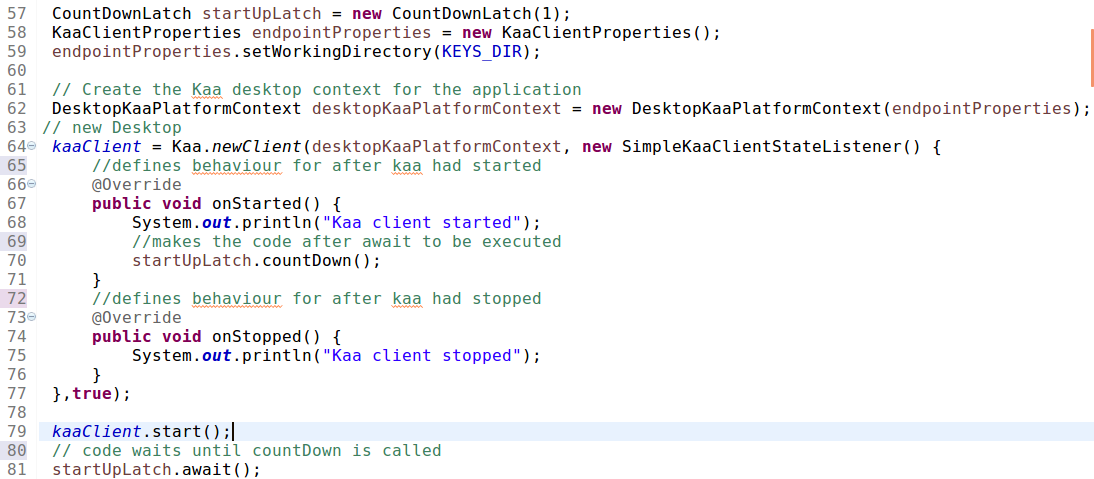
\includegraphics[scale=0.5]{Imagens/start.png}
	\centering  	
  	\captionsource{ C�digo de inicializa��o cliente Kaa
\label{fig:start-event}}{Pr�prio Autor}
  	
\end{figure}
\textbf{
C�digo de Anexa��o da cliente ao usu�rio}

A anexa��o de um cliente a um usu�rio � necess�ria para habilitar o envio/recebimento de eventos, vindo desse cliente, o c�digo na figura \ref{fig:attach} ilustra a opera��o de anexa��o.

\begin{figure}[htb]
	\centering
  	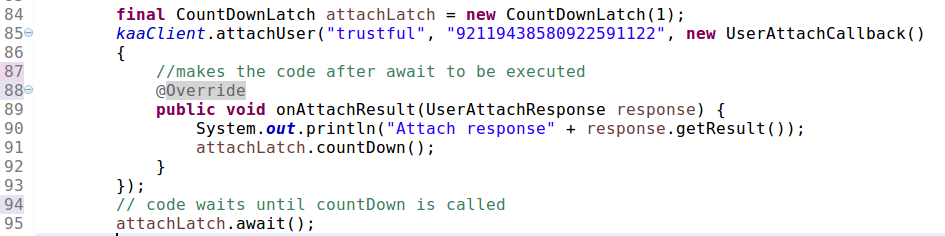
\includegraphics[scale=0.5]{Imagens/attach.png}
	\centering  	
  	\captionsource{ C�digo de anexa��o do usu�rio
\label{fig:attach}}{Pr�prio Autor}
  	
\end{figure}

\textbf{Registro para recebimento de eventos
}
O c�digo na figura \ref{fig:receive} representa o cadastramento do cliente para o recebimento do evento, nesse caso InterruptMeetingEvent e apresenta o comportamento ap�s o recebimento do evento.


\begin{figure}[htb]
	\centering
  	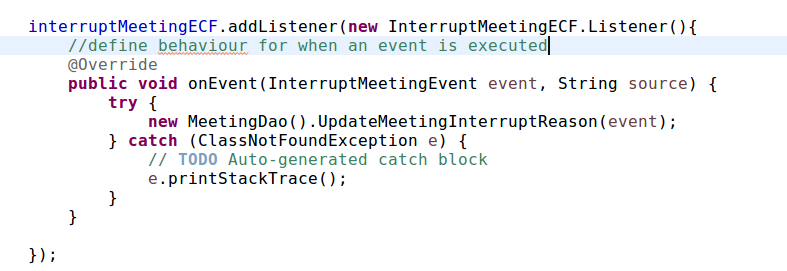
\includegraphics[scale=0.5]{Imagens/receive.png}
	\centering  	
  	\captionsource{ C�digo de registro de recebimento de eventos
\label{fig:receive}}{Pr�prio Autor}
  	
\end{figure}

\textbf{Envio de Eventos} 

O c�digo da figura \ref{fig:send} � utilizado para o envio de um evento. Anteriormente ao envio de um evento � necess�rio saber quais endpoints est�o cadastrados para receber o evento espec�fico, para isso � utilizado o m�todo findEventListeners. Logo ap�s identificado os endpoints pode se enviar o evento para um endpoint espec�fico (unicast) ou para todos os endpoints cadastrados para o recebimento do evento (broadcast). No c�digo apresentado na figura \ref{fig:send} o evento � enviado em modo broadcast.


\begin{figure}[htb]
	\centering
  	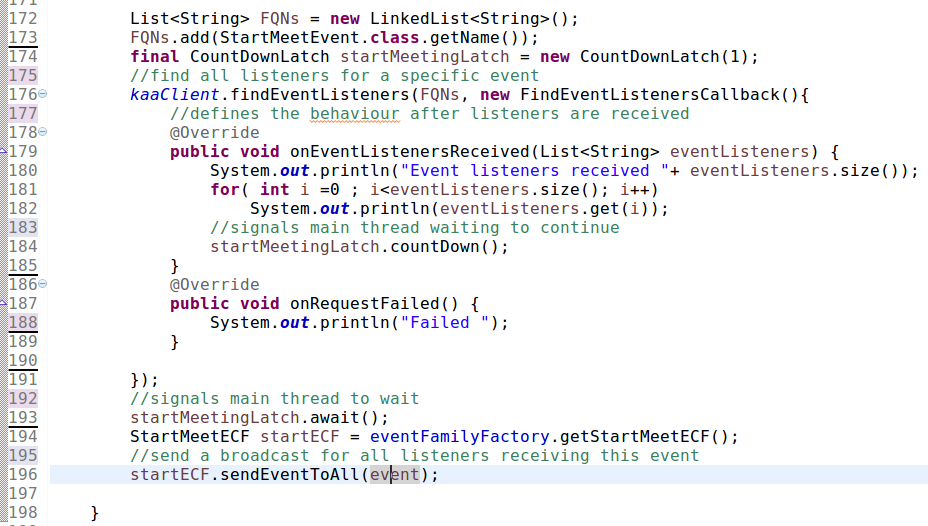
\includegraphics[scale=0.5]{Imagens/send.png}
	\centering  	
  	\captionsource{ C�digo de envio de eventos
\label{fig:send}}{Pr�prio Autor}
  	
\end{figure}

\subsection{Desenvolvimento da aplica��o RoomieRaspberry}
A aplica��o no Raspberry Pi foi feita na linguagem Java e para a interpreta��o dos dados que partiam dos sensores foi utilizada a biblioteca Pi4J. O Raspberry Pi foi escolhido pela a liberdade no uso de linguagens de programa��o e pelo seu maior poder computacional se comparando com outras placas de prototipa��o semelhantes. 
	As principais funcionalidades presentes no RoomieRaspberry s�o a leitura dos dados de sensores RFID e de presen�a; o controle  no fluxo de execu��o da reserva como mostrado no BPM da figura \ref{fig:bpmn} e o recolhimento dos dados para cadastro do usu�rio na plataforma Roomie.

\subsubsection{Diagrama de Classes}

A estrutura do RoomieRaspberry � bem mais simples se comparado com as outras aplica��es Roomie, basicamente as classes utilizadas s�o para realizar a comunica��o com Kaa e para a leitura do sensor RFID. As classes de testes s�o de teste unit�rios das classes da aplica��o.


\begin{figure}[htb]
	\centering
  	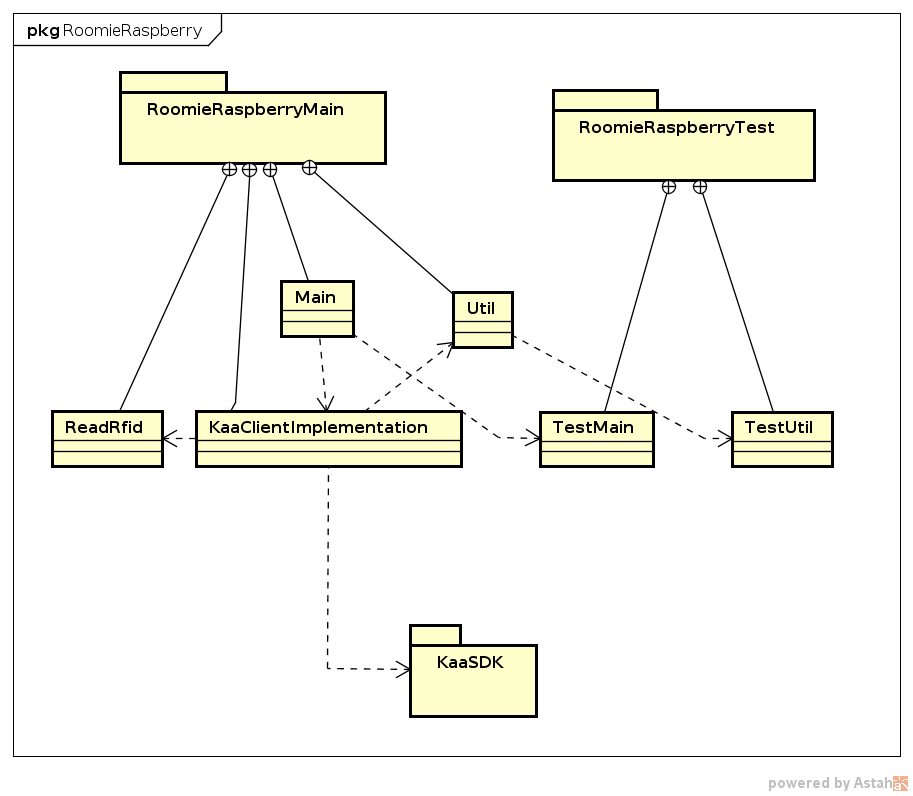
\includegraphics[scale=0.5]{Imagens/roomieraspberry.png}
	\centering  	
  	\captionsource{Diagrama de Classes RoomieRaspberry
\label{fig:class-rasp}}{Pr�prio Autor}
  	
\end{figure}

\subsubsection{Configura��o dos sensores no Raspberry Pi}

Os sensores utilizados para a capta��o dos dados e para sa�da de dados foram os seguintes:
\begin{itemize}
\item Sensor de Presen�a PIR;
\item Leitor cart�o RFID RC522;
\item Leds
\end{itemize}

Para a conex�o com sensores o Raspberry Pi tem uma s�rie de pinos de entrada/sa�da, os chamados GPIO, na figura \ref{fig:pins} � mostrado o mapeamento dos pinos.
Na tabela \ref{TabelaPinos} segue o mapeamento dos pinos que foram usados para a conex�o com os sensores.
  


\begin{figure}[htb]
	\centering
  	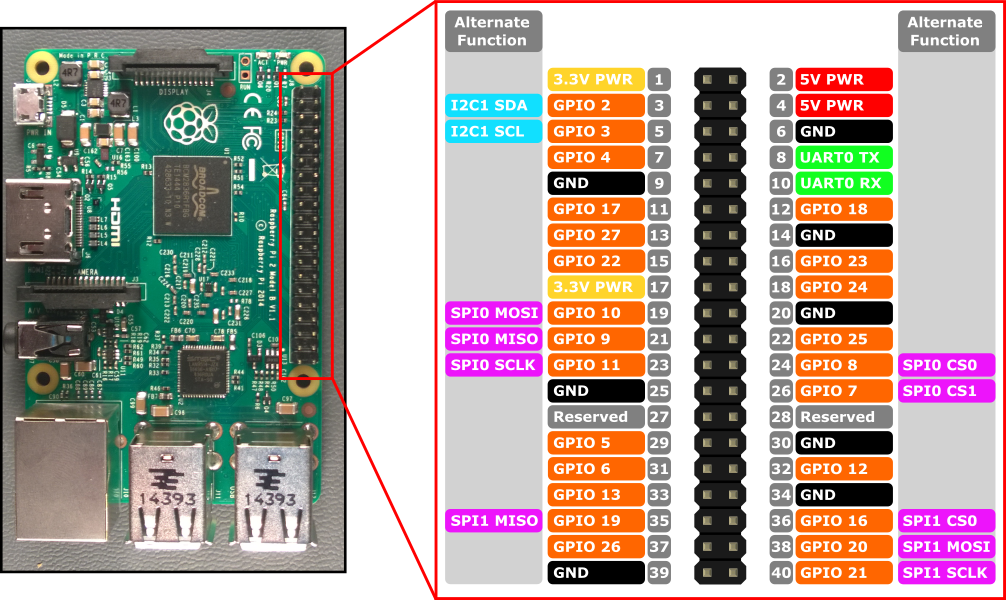
\includegraphics[scale=1.5]{Imagens/pins.png}
	\centering  	
  	\captionsource{ Mapeamento dos pinos do Raspberry Pi 2 e 3
\label{fig:pins}}{\cite{microsoft}}
  	
\end{figure}


\begin{table}
\begin{center}
\begin{tabular}{ | c | c | c |}
\hline
\thead{Sensor/Pino}&\thead{Numera��o Pino Raspberry}&\thead{Pino GPIO}\\ \hline
RC522/SDA&24&\makecell{GPIO8}\\ \hline
RC522/SCK&23&\makecell{GPIO11}\\ \hline
RC522/MOSI&19&\makecell{GPIO10}\\ \hline
RC522/MISO&21&\makecell{GPIO9}\\ \hline
RC522/GND&20&\makecell{GND}\\ \hline
RC522/3.3V&1&\makecell{3V3}\\ \hline
PIR/VCC&2&\makecell{5V3}\\ \hline
PIR/GND&6&\makecell{GND}\\ \hline
PIR/OUT&16&\makecell{GIPO(23)}\\ \hline
Led Vermelho&7&\makecell{GPIO 04}\\ \hline
Led Verde&11&\makecell{GPIO 17}\\ \hline
Led Amarelo&13&\makecell{GPIO 27}\\ \hline
\end{tabular}
\end{center}
\caption{ Mapeamento de pinos para o Raspberry Pi}
\label{tab:TabelaPinos}
\end{table}

Os Leds Coloridos s�o utilizados no fluxo de execu��o da reserva, um led por vez � acesso representando um est�gio no fluxo de reserva.
\begin{itemize}

\item Vermelho: N�o existe reserva no momento.
\item Amarelo: Reserva identificada e sala pronta para a identifica��o do RFID.
\item Verde: indica que o cart�o RFID foi liberado e que a sala est� liberada.

\end{itemize} 

\subsection{Desenvolvimento do RoomieWeb }

A aplica��o RoomieWeb foi desenvolvida utilizando a linguagem Java e o framework Spring MVC. O principal objetivo da aplica��o � fornecer uma interface amig�vel para os usu�rios gerenciarem suas reservas. 

\subsubsection{Diagrama de Classes 
}
A Figura \ref{fig:roomieweb} apresenta o diagrama de classes do RoomieWeb, como mencionado anteriormente � utilizado o modelo arquitetural MVC com adi��o de um pacote de Objeto de Acesso a Dados tamb�m chamado DAO (Data Access Object) para promover o desacoplamento das classes que lidam com banco de dados. As classes de teste no diagrama s�o classes utilizadas para testes unit�rios da aplica��o.

\begin{figure}[htb]
	\centering
  	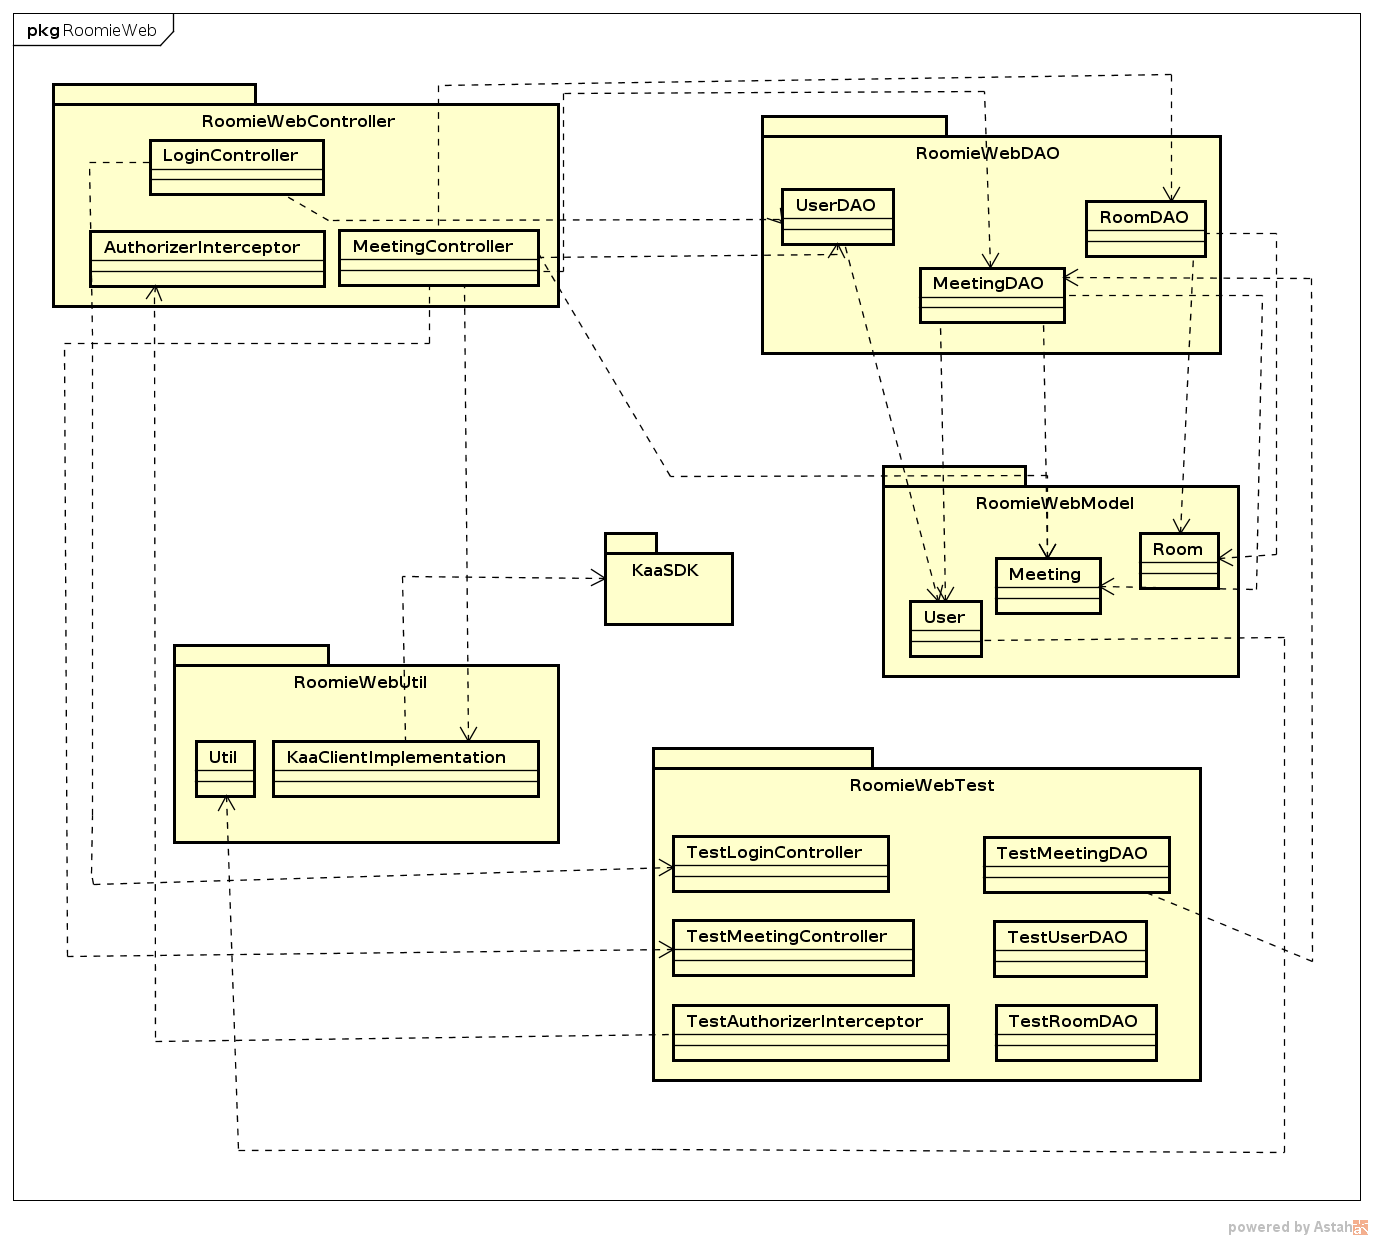
\includegraphics[scale=0.5]{Imagens/roomieweb.png}
	\centering  	
\captionsource{ Diagrama de classes RoomieWeb 
\label{fig:roomieweb}}{Pr�prio Autor}
  	
\end{figure}

\subsection{Principais Telas da Aplica��o}

\textbf{Login}
A figura \ref{fig:login} representa a tela inicial de login da aplica��o RoomieWeb, nessa tela usu�rios que j� est�o cadastrado no sistema Roomie podem ter acesso a plataforma.\\

\begin{figure}[htb]
	\centering
  	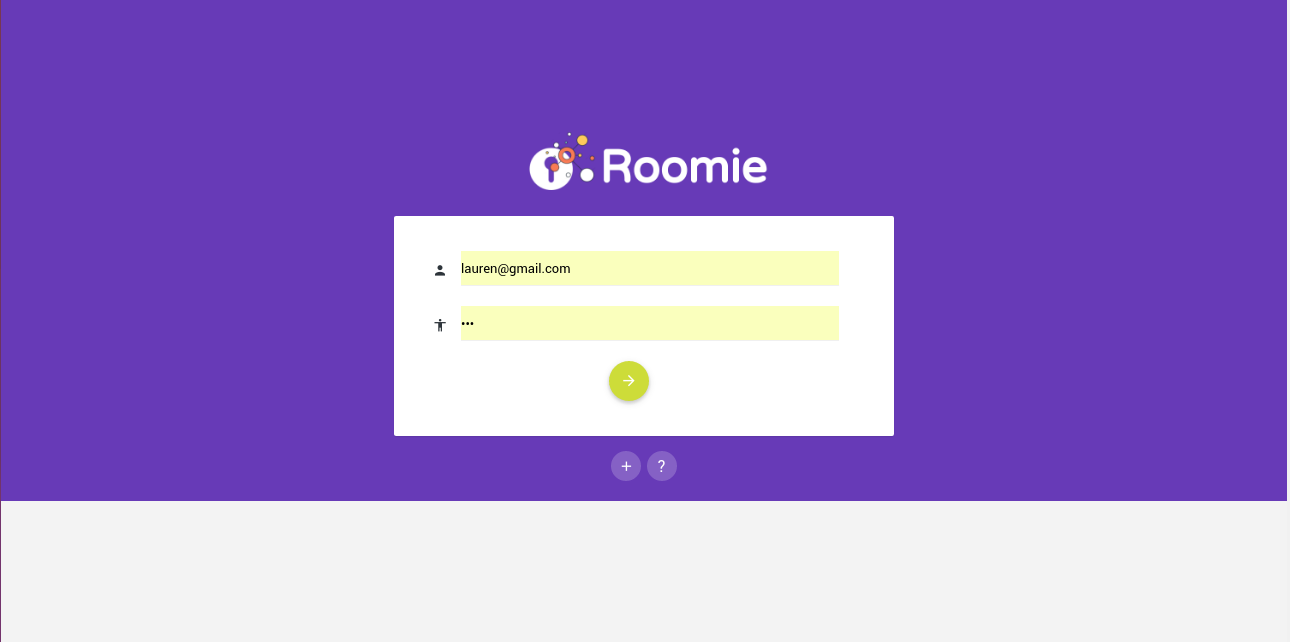
\includegraphics[scale=0.5]{Imagens/login.png}
	\centering  	
\captionsource{Tela de Login RoomieWeb 
\label{fig:login}}{Pr�prio Autor}
  	
\end{figure}

\textbf{Cria��o de nova reuni�o}


A figura \ref{fig:createmeeting} representa a tela da cria��o de nova reservas na aplica��o RoomieWeb, nessa tela o usu�rio pode criar uma nova reserva no RoomieWeb. Os campos de salas e usu�rios s�o populados diretamente do banco de dados.\\ 
\begin{figure}[htb]
	\centering
  	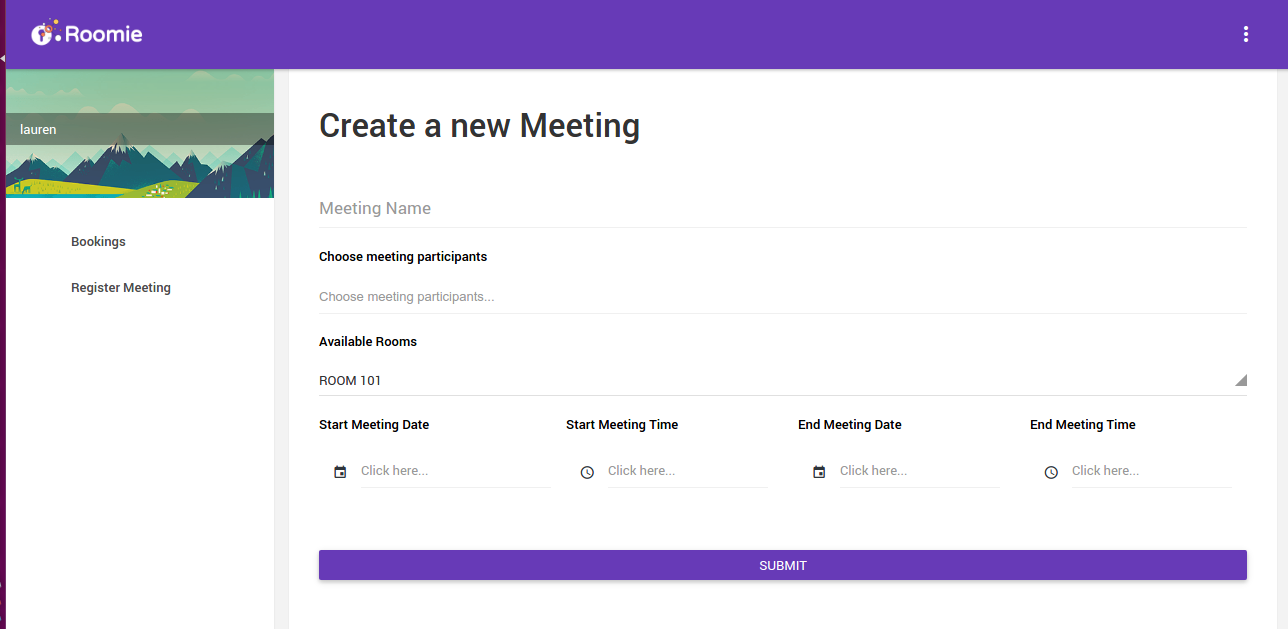
\includegraphics[scale=0.5]{Imagens/createmeeting.png}
	\centering  	
\captionsource{Tela de Login RoomieWeb 
\label{fig:createmeeting}}{Pr�prio Autor}
  	
\end{figure}


\textbf{Visualiza��o/Edi��o de Reservas}
A figura \ref{fig:showmeetings} representa a tela de listagem de todas as reuni�es que o usu�rio logado no momento participa, caso o usu�rio seja o criador da reserva tamb�m � poss�vel realizar a edi��o/exclus�o da reserva.\\

\begin{figure}[htb]
	\centering
  	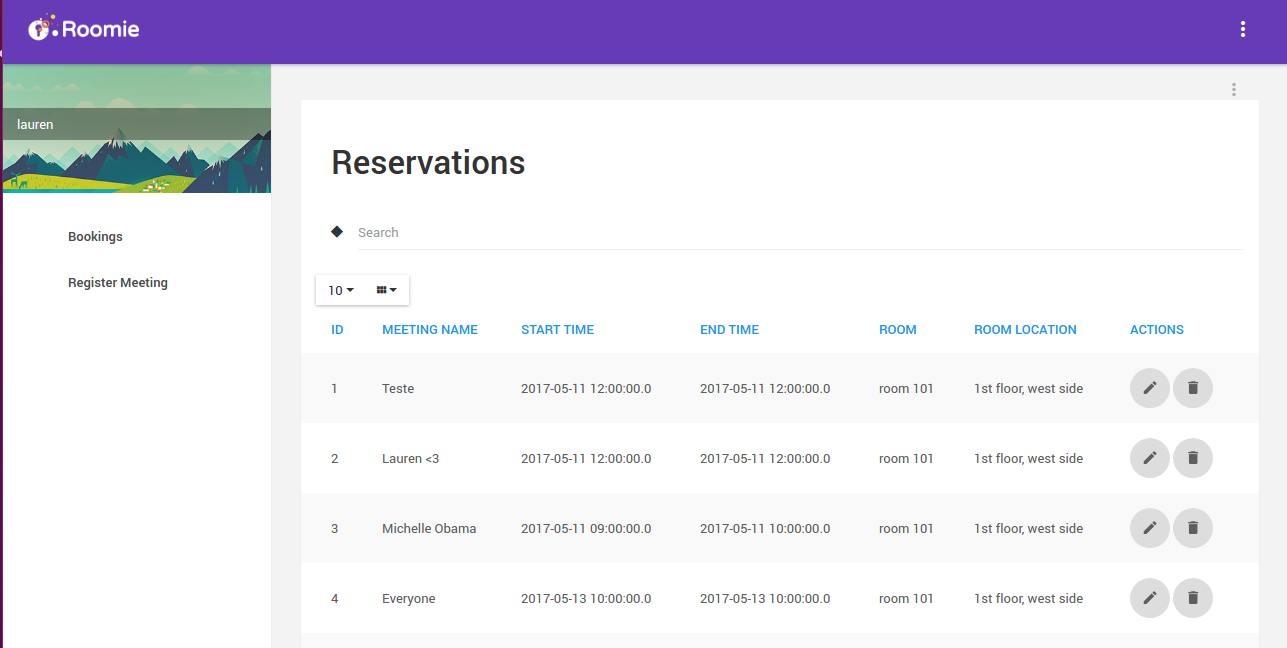
\includegraphics[scale=0.5]{Imagens/showmeetings.png}
	\centering  	
\captionsource{Listagem de reuni�es do usu�rio 
\label{fig:showmeetings}}{Pr�prio Autor}
  	
\end{figure}


\subsubsection{Desenvolvimento do RoomieController}

A Aplica��o RoomieController tem como principal objetivo gerenciar o sistema como um todo, ou seja, � a entidade respons�vel por diversas atividades que permitem que aplica��o funcione corretamente. A aplica��o RoomieController recupera as informa��es necess�rias para o funcionamento da aplica��o RoomieRaspberry e tamb�m gerenciar o disparo de eventos de in�cio de reuni�es. Na Figura \ref{fig:roomiecontroller} � mostrado o diagrama de classes da aplica��o.


\begin{figure}[htb]
	\centering
  	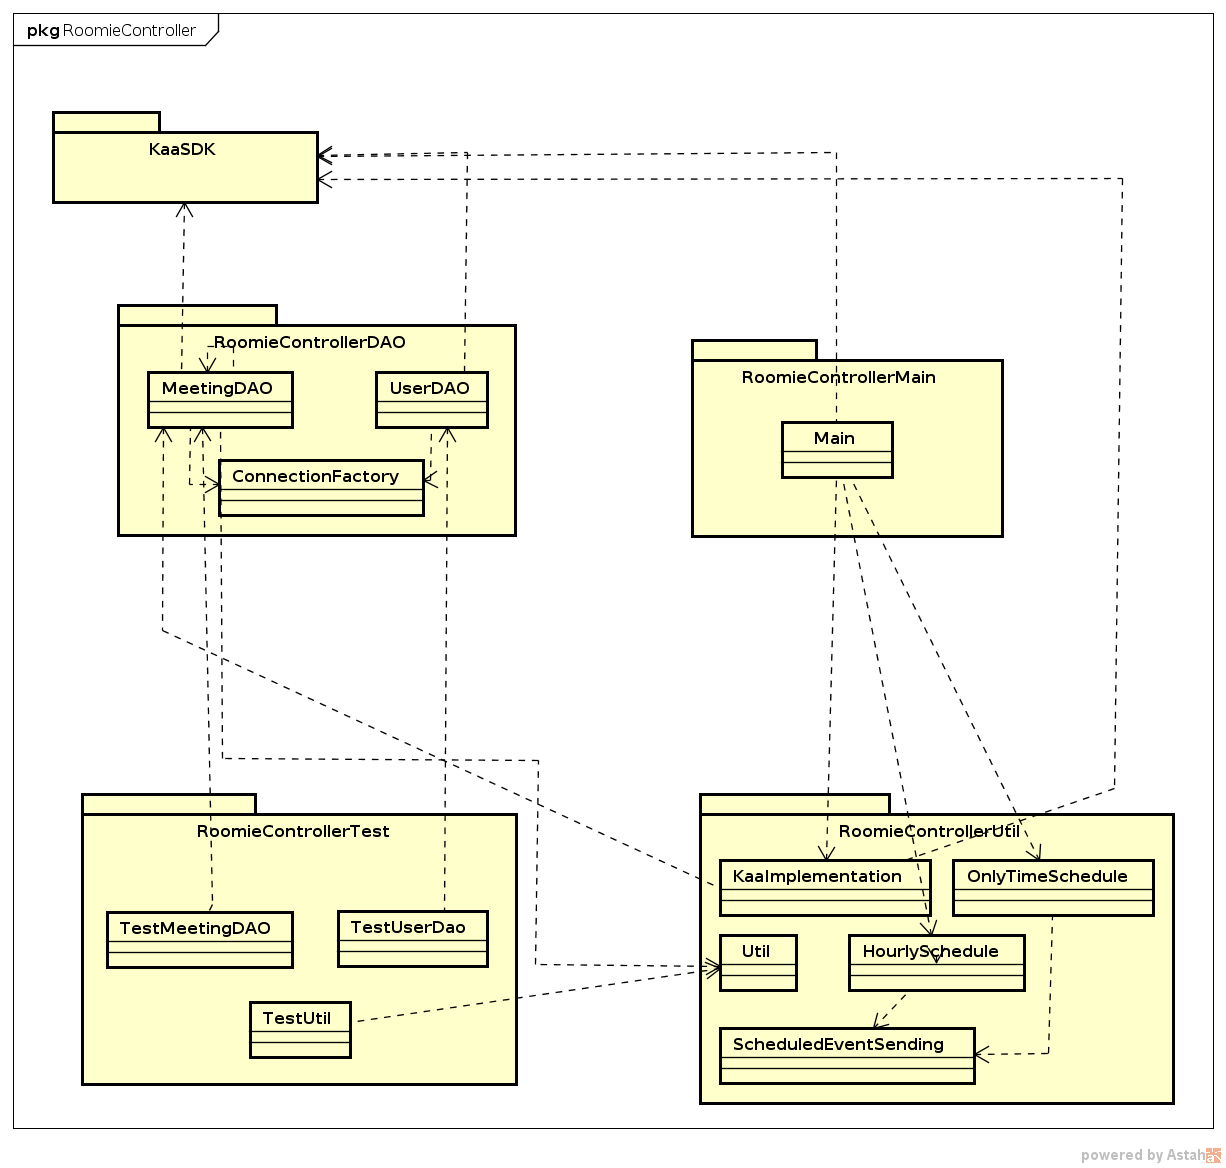
\includegraphics[scale=0.5]{Imagens/roomiecontroller.png}
	\centering  	
\captionsource{Diagrama de Classes RoomieController
\label{fig:roomiecontroller}}{Pr�prio Autor}
  	
\end{figure}



\subsection{Execu��o Final da Aplica��o}
Para o teste final do sistema Roomie, foi feito um experimento em uma sala de reuni�o durante 2 horas. O roteiro do teste foi feito para que grande parte das possibilidades e situa��es diferentes fossem testadas.
	Foram utilizados tr�s personagens no cen�rio: Lauren, Alex e Camila. Os tr�s tinham diferentes cart�es rfids e cadastros separados na aplica��o. A tabela \ref{tab:TabelaTestes} cont�m as reuni�es que foram criadas e mais informa��es sobre cada reuni�o.



\begin{table}

\begin{tabular}{ | c | c | c | c |}
\hline

\thead{Nome da Reuni�o}&\thead{Hor�rio }&\thead{Participantes}&\thead{Descri��o do Cen�rio}\\ \hline
Lauren - Individual&\makecell{09:00-09:15}&Lauren&
\makecell{09:03 - Lauren recebe um email\\ informando 
que caso n�o compare�a a sala \\
sua reserva ser� cancelada.\\
09:03:30 Lauren entra na sala \\com seu cart�o RFID e tem \\acesso permitido.}\\ \hline
Plano de A��o&09:20 - 09:45&\makecell{Lauren, Alex}&\makecell{Lauren convida Camila \\para a reuni�o mas n�o edita a reserva.\\ 09:20 -Camila chega na sala,\\ mas n�o consegue se autenticar \\com seu cart�o RFID.
\\09:22 - Alex chega na reuni�o\\ cart�o RFID e tem acesso liberado.}\\ \hline
1:1 Camila e Alex&10:00 -10:30&\makecell{Camila, Alex}&\makecell{\\10:00 - Ambos chegam na reuni�o as 10:00 \\ap�s 15 min a reuni�o � finalizada, \\mas os participantes n�o cancelam a \\reserva no sistema.
\\10:20 - Reuni�o � automaticamente \\ cancelada}\\ \hline
Camila - Individual&10:40-11:10&\makecell{Camila}&
\makecell{10:46 - Camila recebe email \\avisando que sua reserva ser� \\ cancelada caso n�o \\compare�a at� �s 10:49.\\
10:50 - Camila tenta entrar\\ nas sala mas n�o consegue\\ autenticar com seu cart�o.}
\\ \hline

\end{tabular}
\caption{Tabela de casos de teste}
\label{tab:TabelaTestes}
\end{table}

%\hyperref[video]{''http://bit.ly/2rGTlRp''}
V�deo de execu��o da aplica��o
%We use \hyperref[video]{lemma \ref*{video} }

	
	% Capitulo 5: Quinto cap�tulo (arquivo Includes/Capitulo5.tex)
	%% Cap�tulo 5
\chapter{Cap�tulo 5}

\section{Se��o 1}

Se��o 1


\section{Se��o 2}

Alguns exemplos de cita��o: 

Na tese de Doutorado de Paquete \cite{PaquetePhD}, discute-se sobre algoritmos de busca local estoc�sticos aplicados a problemas de Otimiza��o Combinat�ria considerando m�ltiplos objetivos. Por sua vez, o trabalho de \cite{KnowlesBoundedLebesgue}, publicado nos anais do IEEE CEC de 2003, mostra uma t�cnica de arquivamento tamb�m empregada no desenvolvimento de algoritmos evolucion�rios multi-objetivo, trabalho esse posteriormente estendido para um cap�tulo de livro dos mesmos autores \cite{KnowlesBoundedPareto}. Por fim, no relat�rio t�cnico de \citeonline{Jaszkiewicz}, fala-se sobre um algoritmo gen�tico h�brido para problemas multi-crit�rio, enquanto no artigo de jornal de Lopez \textit{et al.} \cite{LopezPaqueteStu} trata-se do \textit{trade-off} entre algoritmos gen�ticos e metodologias de busca local, tamb�m aplicados no contexto multi-crit�rio e relacionado de alguma forma ao trabalho de Jaszkiewicz (\citeyear{Jaszkiewicz}).

Outros exemplos relacionados encontram-se em \cite{Silberschatz} (livro),  (refer�ncia da Web) (disserta��o de Mestrado).

\subsection{Subse��o 5.1}

Subse��o 5.1


\subsection{Subse��o 5.2}

Subsection 5.2


\section{Se��o 3}

Se��o 3
		
	% Consideracoes finais
	% Considera��es finais
\chapter{Considera��es finais}

\section{Trabalhos Futuros}
	
	% Bibliografia (arquivo Capitulos/Referencias.bib)
	\bibliography{Capitulos/Referencias}
	\bibliographystyle{abnt-alf}
	
	% Ap�ndice A (arquivo Includes/ApendiceA)
	% Ap�ndice
\apendice
\chapter{Primeiro ap�ndice}

Os ap�ndices s�o textos ou documentos elaborados pelo autor, a fim de complementar sua argumenta��o, sem preju�zo da unidade nuclear do trabalho.
	
	% P�gina em branco
	\newpage

\end{document}